%% =====================================================================
%%  Elsevier CAS double-column manuscript (cas-dc.cls)
%%  Ported from the elsarticle preprint version.
%%  Build:  pdflatex cas-main -> bibtex cas-main -> pdflatex cas-main x2
%% =====================================================================
\documentclass[a4paper,fleqn]{cas-dc}

\usepackage[numbers]{natbib}
\usepackage{amsmath,amssymb,amsthm,mathtools}
\usepackage{booktabs}
\usepackage{tabularx}
\usepackage{multirow}
\usepackage{array}
\usepackage[capitalise,noabbrev]{cleveref}
\crefname{hypothesis}{Hypothesis}{Hypotheses}
\crefname{remark}{Remark}{Remarks}
\crefname{corollary}{Corollary}{Corollaries}
\crefname{proposition}{Proposition}{Propositions}

\newtheorem{theorem}{Theorem}[section]
\newtheorem{lemma}[theorem]{Lemma}
\newtheorem{proposition}[theorem]{Proposition}
\newtheorem{corollary}[theorem]{Corollary}
\theoremstyle{definition}
\newtheorem{definition}[theorem]{Definition}
\newtheorem{hypothesis}{Hypothesis}
\newtheorem{remark}[theorem]{Remark}
\renewcommand{\proofname}{Proof}

\newcommand{\R}{\mathbb{R}}
\newcommand{\E}{\mathbb{E}}
\newcommand{\PP}{\mathbb{P}}
\newcommand{\norm}[1]{\left\lVert#1\right\rVert}
\newcommand{\holder}[1]{\norm{#1}_{\gamma}}
\newcommand{\dd}{\,\mathrm{d}}

\setlength{\emergencystretch}{3em}

\begin{document}
\let\WriteBookmarks\relax
\def\floatpagepagefraction{1}
\def\textpagefraction{.001}

\shorttitle{Almost sure averaging with learned drift}
\shortauthors{W. Wang et~al.}

\title[mode=title]{Almost sure averaging for discrete stochastic systems with
learned drift: trajectory-level error decomposition in denoising diffusion samplers}

\author[1,2,3]{Wei Wang}
\cormark[1]
\ead{wangwei@lntu.edu.cn}

\author[3]{Yiran Chang}

\author[2]{Fei Ding}


\affiliation[1]{organization={Foundation Department, Liaoning Technical University},
            country={China}}

\affiliation[2]{organization={Anhui Engineering Research Center for Intelligent
            Computing and Information Innovation, Fuyang Normal University},
            country={China}}

\affiliation[3]{organization={School of Electronic and Information Engineering,
            Liaoning Technical University},
            country={China}}

\cortext[1]{Corresponding author.\ E-mail: wangwei@lntu.edu.cn}

\begin{abstract}
Convergence theories for denoising diffusion samplers are largely
distribution-based: they bound the distance between the output and the target
probability law but provide little information about individual simulated
trajectories, which the step size and the schedule parameters must regulate. We
seek a trajectory-level theory that attributes observed errors to distinct
sources. We treat diffusion samplers as discrete fast--slow stochastic systems
equipped with a fast-time-fluctuating learned drift and apply almost sure
diffusion-approximation tools from averaging theory. Under polynomial decay of
the mixing coefficients of the driving noise we obtain H\"older-norm bounds on
the trajectory error and transfer the pathwise estimates to the terminal law by
a coupling argument. The forward chain embeds into the averaging scheme with
per-step $O(N^{-2})$ deterministic remainders that accumulate to $O(N^{-1})$ on
$[0,T]$, and its paths converge almost surely at rate $N^{-\alpha}$ for every
$\alpha<1/2-\gamma$. The reverse-process error decomposes into three
interpretable contributions: fast-scale averaging, learned-drift approximation
and time discretisation. A spectral criterion identifies the drift frequencies
that window averaging cannot remove, and an \emph{a posteriori} computable
diagnostic $\mathrm{osc}(N)$ detects that failure. When the fast-scale error
dominates, refining the step size yields limited benefit and modulating the
noise schedule becomes the effective intervention. Numerical illustrations with
bootstrap $95\%$ confidence intervals validate the predicted scaling laws.
\end{abstract}

\begin{highlights}
\item Diffusion samplers are analysed as discrete fast--slow stochastic systems.
\item The forward chain embeds in an averaging scheme with per-step $O(N^{-2})$ remainders.
\item A H\"older bound gives pathwise almost sure convergence at an explicit rate.
\item A spectral criterion identifies drift frequencies unaffected by window averaging.
\item A trained-network diagnostic detects averaging breakdown; schedule modulation helps.
\end{highlights}

\begin{keywords}
Multiscale stochastic systems \sep Averaging principle \sep Almost sure pathwise
convergence \sep H\"older regularity \sep Learned drift \sep Weak dependence
\end{keywords}

\maketitle

\section{Introduction}
\label{sec:intro}

The averaging principle is the classical tool for systems with two separated time
scales. When a slow variable is driven by a rapidly fluctuating, weakly dependent
perturbation, the fast degrees of freedom are eliminated in the limit of infinite
scale separation, and the slow variable is described by an effective equation whose
coefficients are averages of the original ones against the invariant law of the fast
variable, with an error controlled by the mixing rate of the latter
\citep{bogoliubov1961,khasminskii1966,papanicolaou1977,bensoussan1978,freidlin2012,
pavliotis2008,givon2004,dolgopyat2004}. The principle has two flavours that are often
conflated. In its \emph{distributional} form it identifies the limit law of the slow
variable. In its \emph{pathwise}, or \emph{almost sure}, form it compares, on a single
probability space and for a single realisation of the driving noise, the trajectory of
the multiscale system with that of the effective equation. The second form is
considerably stronger, and it is the form required by numerical practice: a simulation
produces one path, not an ensemble, and the way in which the error accumulates along
that path cannot be read off a statement about laws.

Pathwise approximation for dependent sequences has a long history, from strong
invariance principles \citep{strassen1964} through almost sure invariance principles
for mixing and weakly dependent sequences \citep{philipp1975,berkes1979,bradley2005,
wu2005} to the martingale moment inequalities on which the argument below rests
\citep{hall1980}. For diffusion approximation in continuous time the pathwise
statement was obtained by rough path techniques \citep{friz2024} and, more recently,
re-derived through a deterministic-estimate framework that dispenses with rough paths
and yields a H\"older-norm bound directly \citep{kifer2025}. The latter is the tool
used here, for two reasons: its hypotheses --- stationarity and polynomial decay of
mixing coefficients, bounded Lipschitz coefficients --- are checkable in the present
setting, and its conclusion is stated in the topology in which we wish to compare
paths.

Two features of the existing literature motivate what follows. First, the worked
examples of averaging are largely physical --- Langevin dynamics with fast
thermal noise, climate models with fast weather fluctuations, molecular dynamics with fast
vibrations --- and in each case the drift is a known function of the state. Second,
when the drift is instead a \emph{learned} function of state and time, it is neither
known analytically nor guaranteed to be regular in time, and its error is correlated
across neighbouring steps because it is produced by the same network evaluated at
nearby inputs. Discrete-time stochastic systems of this type have, to our knowledge,
not been analysed within the almost sure averaging framework. That is the gap
addressed here, with a specific and widely used instance as the test case.

A denoising diffusion model defines a forward chain that progressively perturbs data
into noise,
\begin{equation}
x_{k+1} = \sqrt{1-\beta_{k}}\,x_{k} + \sqrt{\beta_{k}}\,\varepsilon_{k},
\qquad \varepsilon_{k}\sim\mathcal{N}(0,I_{d}),
\label{eq:ddpm-forward}
\end{equation}
together with a reverse chain that integrates a learned drift backwards in time and
transports noise into data \citep{sohl2015,ho2020,song2021sde}. Equation
\eqref{eq:ddpm-forward} is the Euler--Maruyama discretisation of an
Ornstein--Uhlenbeck-type diffusion with a time-inhomogeneous coefficient, and the
reverse chain is the same object with the arrow of time reversed. Two time scales are
visible in this reading: the slow scale $t=k/N$ on which the marginal law migrates
from data to noise, and the fast scale on which the injected noise decorrelates. A
sampler is thus a discrete fast--slow scheme, and the object whose error a user
observes is a single trajectory of that scheme. Read as a multiscale system, however,
it differs from the classical examples in three respects, each of which is a genuine
obstruction rather than a notational inconvenience.

The first is that the drift depends on the fast phase as well as on the slow state.
The score field is evaluated at $(x_{k},k/N)$, and its dependence on the second
argument is fixed by the network architecture --- in particular by the frequency
content of the time embedding --- rather than by a known physical law. The
scale-separation condition that the averaging principle requires is therefore a
statement about a trained object, not about a model. The second is that the drift
error is weakly dependent, not independent: successive score evaluations share
parameters and act on nearby inputs, so their errors are correlated, and the averaging
residual does not decay at the $M^{-1/2}$ rate that an independence assumption would
suggest. The third is that the dimension is high and the state space is unbounded: a
global Lipschitz constant is unavailable for the score of any target with unbounded
support, so interior path estimates must be separated from exit events. These three
points set the technical agenda: an embedding exact enough to transfer the available
theory (\Cref{sec:setting}), a trajectory-level bound that survives the weak
dependence of the learned field (\Cref{sec:main}), and an explicit treatment of the
scale-separation hypothesis including the case in which it fails
(Remark~\ref{rem:H-fail-consequence}, \Cref{sec:exp-e4,sec:exp-e6}).

The literature that this agenda touches is split across two communities, and the gap
lies between them. On the probabilistic side the tools are mature, and the present
paper does not claim to improve them; what is missing there is not a rate but a
transfer. The averaging theory is stated for coefficients that are known, bounded and
Lipschitz in both arguments, and the deterministic-estimate route of Kifer
\cite{kifer2025} requires control of the drift's temporal oscillation over a window of
the fast scale. Neither requirement is automatic for a learned field, and neither is
discussed in the multiscale literature. The same applies to the Poisson-equation route
to averaging, which quantifies the corrector through the solution of an auxiliary
equation \citep{pardoux2001}: the estimates there are stated for analytic
coefficients, and an error bound for a drift that is only accessible through the
parameters of a trained network is not available.

On the generative-modelling side the available convergence theory is almost entirely
distributional. Building on the reverse-time representation of Anderson
\cite{anderson1982}, a sequence of works established non-asymptotic bounds in total
variation, Kullback--Leibler divergence and Wasserstein distance under progressively
weaker assumptions on the data law and on the score estimate
\citep{block2020,lee2023convergence,chen2023sampling,debortoli2022,benton2024linear,
li2025odt}. The sharpest of these give an $O(d/T)$ total-variation bound, refined to
$O(k/T)$ with $k$ the intrinsic dimension, under assumptions as mild as a finite first
moment \citep{li2025odt}. This line of work answers, essentially completely, how many
steps are needed for the marginal law to be accurate, and we use it only as a
benchmark for what a pathwise statement can add. Trajectory-level statements are not
absent, but they are of a different kind. Classical strong convergence of the
Euler--Maruyama scheme gives pathwise $L^{p}$ rates for globally Lipschitz
coefficients \citep{kloeden1992,milstein1995,higham2001}; coupling arguments transfer
these to the diffusion setting; and flow-map approaches learn the It\^o map itself
with explicit pathwise guarantees. Every one of these yields \emph{a total error
bound}. Sampler design, by contrast, needs \emph{a decomposition of that bound into
terms attributable to distinct mechanisms} --- the residual oscillation of the fast
scale, the imperfection of the learned drift, and the finiteness of the step size.
Without such a decomposition one cannot tell whether an observed discrepancy between
prediction and measurement comes from the schedule, from the network, or from the
discretisation, and therefore cannot address it. In short, the available
sampling theory is distributional and attributes nothing, while the available
averaging theory is pathwise but stated for analytic drifts, and no embedding that is
exact to the correct order has been given for a time-fluctuating learned field.

We address it with an exact embedding, a trajectory-level bound and a decomposition of
the resulting error. The embedding (Proposition~\ref{prop:embedding}) identifies the
forward chain \eqref{eq:ddpm-forward} with the discrete fast--slow scheme of Kifer
\cite{kifer2025} up to a deterministic remainder that is $O(N^{-2})$ per step and
$O(N^{-1})$ on $[0,T]$, with the noise sequence in the role of the fast variable. The
two orders must not be conflated: a per-step remainder of order $N^{-2}$ accumulates
over $N$ steps, so a statement that reports only the per-step order is off by one power
of $N$ at the level of the trajectory, and \Cref{sec:exp-e2} measures the accumulated
order directly. The same comparison yields the trajectory-level bound
(\Cref{thm:forward}): under polynomial decay of the mixing coefficients with exponent
$\beta>2$ and bounded Lipschitz coefficients, the H\"older norm of the trajectory error
is $O(N^{-(1/2-\gamma)})$ in expectation, and the trajectories converge almost surely
at rate $N^{-\alpha}$ for every $\alpha<1/2-\gamma$. The rate is inherited from the
averaging framework of Kifer \cite{kifer2025}; what is new is its applicability to a
learned, time-fluctuating discrete system, together with the decomposition below, not
the probabilistic rate itself.

The decomposition that the argument calls for follows from the same estimates. The
reverse-process error separates into a fast-scale averaging term, a score term and a
discretisation term (Corollary~\ref{cor:rule}, \Cref{thm:decomp}), and the relative
size of the first two decides whether refining $\Delta t$ or modulating the noise
schedule --- the macroscopic modulation of the multiscale system --- is the effective
intervention. The hypothesis that carries the argument is then stated in a form that
can be checked (Hypothesis~\ref{hyp:H}, Proposition~\ref{prop:H-suff},
Proposition~\ref{prop:H-fail}, Remark~\ref{rem:H-fail-consequence}): the assumption
that the learned field averages over a window of the fast scale is made explicit;
three sufficient conditions are given with explicit moduli and an optimal window
exponent; a spectral criterion (Proposition~\ref{prop:spectral}) identifies exactly
which temporal frequencies of the drift are invisible to the window average, and shows
that the aliasing counterexample is the resonant case of that criterion; and a
diagnostic $\mathrm{osc}(N)$, computable \emph{a posteriori} on any trained network,
detects failure. The hypothesis is \emph{not} derived from the score-matching training
loss; that remains open for learned drift fields, as discussed in
Remark~\ref{rem:H-scope}. A coupling argument carries the pathwise statement to the
terminal law (\Cref{thm:dist}): together with an explicit initialisation estimate, it
converts the trajectory bound into a $W_{1}$ bound whose every term is attached to the
same named mechanism, which is what connects the dynamical statement to the
distributional statements that the sampling literature reports, and it is obtained
without additional density assumptions. A numerical study complements the results
(\Cref{sec:numerics}): a synthetic fast--slow system, an analytic-score sampler and a
trained score network are used to measure the predicted orders, the three terms
separately, the two branches of the design rule, and the diagnostic on a real learned
drift field.

Two limitations follow from the structure just described. When the driving noise is
independent --- the standard denoising chain --- the averaging structure degenerates,
\eqref{eq:rate-forward} reduces to the classical strong convergence of the
Euler--Maruyama scheme, and no new rate is obtained; the framework becomes informative
when the noise is weakly dependent or, more relevant in practice, when the learned
drift fluctuates on the fast scale (Remark~\ref{rem:degenerate}). We claim neither
distributional optimality nor sharp constants: the bounds are stated as scaling laws,
with constants that depend on the data and are not optimised (Remark~\ref{rem:dist}).
The degenerate case is thus part of the statement rather than an excluded
configuration, and the hypothesis that carries the argument is stated in a form that
can be checked, and can fail. Throughout, $\holder{\cdot}$ denotes the
$\gamma$-H\"older norm on $C([0,T];\R^{d})$, $\gamma\in(0,1/2)$, given by
$\holder{f}=\sup_{t}\lvert f(t)\rvert+\sup_{s\ne t}\lvert f(t)-f(s)\rvert/\lvert t-s\rvert^{\gamma}$;
$\Delta t=T/N$; and
$C,C_{1},C_{2},\dots$ are constants independent of $N$ whose values may change between
lines. We call $s_{\theta}$ the \emph{learned drift field}; in the machine learning
literature the same object is called the \emph{score}, and we write ``score''
parenthetically where the connection matters. The map $t\mapsto\beta(t)$ is the
\emph{noise schedule} of that literature; dynamically it is the macroscopic modulation
of the fast scale, and we use both readings. ``Convergence'' always means \emph{pathwise
almost sure convergence in H\"older topology} unless the classical strong convergence
of the Euler--Maruyama scheme is explicitly under discussion. \Cref{sec:setting} establishes
the scheme and the assumptions, \Cref{sec:main} states the results,
\Cref{sec:numerics} reports the numerical protocol, \Cref{sec:discussion} discusses
limitations, and \Cref{app:proofs} collects the proofs.
%% =====================================================================
\section{Problem setting and assumptions}
\label{sec:setting}
%% =====================================================================

\subsection{The discrete fast--slow scheme}

\begin{definition}[Discrete fast--slow scheme, cf.\ \cite{kifer2025}]
\label{def:scheme}
Let $\xi=(\xi_{k})_{k\ge 0}$ be a centred stationary $\R^{m}$-valued process and let
$b:\R^{d}\to\R^{d}$, $\sigma:\R^{d}\to\R^{d\times m}$ be smooth. For $N\in\mathbb{N}$
define $X^{N}_{0}=x_{0}$ and
\begin{equation}
X^{N}_{k+1} = X^{N}_{k} + \frac{1}{N}\,b\bigl(X^{N}_{k}\bigr)
+ \frac{1}{\sqrt{N}}\,\sigma\bigl(X^{N}_{k}\bigr)\,\xi_{k}
\label{eq:scheme}
\end{equation}
for $k=0,\dots,\lfloor NT\rfloor-1$.
\end{definition}

The fast time scale is $k\mapsto k/N$: as $N$ grows, the perturbation
$N^{-1/2}\sigma\xi_{k}$ accumulates into a diffusion while its individual increments
shrink. The averaging principle asserts that $X^{N}$ approaches, in a sense to be
made precise, the diffusion
\begin{equation}
\begin{split}
\dd \bar X_{t} &= \bar b\bigl(\bar X_{t}\bigr)\dd t + \bar\sigma\bigl(\bar X_{t}\bigr)\dd W_{t},\\
\bar a(x) &:= \sum_{k\in\mathbb{Z}} \E\bigl[\sigma(x)\xi_{0}\,\xi_{k}^{\top}\sigma(x)^{\top}\bigr],
\end{split}
\label{eq:limit}
\end{equation}
with $\bar b$ the average of $b$ against the invariant law of $\xi$; when $\xi$ is
i.i.d.\ centred, $\bar a = \sigma\sigma^{\top}$ and $\bar b = b$.

\subsection{Weak dependence}

\begin{hypothesis}[Mixing]
\label{hyp:mixing}
$\xi$ is stationary and centred with $\E\lvert\xi_{0}\rvert^{2+\delta}<\infty$ for
some $\delta>0$, and its strong mixing coefficients satisfy
$\alpha(k)\le C_{\alpha}(1+k)^{-\beta}$ for some $\beta>1$.
\end{hypothesis}

\begin{hypothesis}[Regularity]
\label{hyp:regular}
$b$ and $\sigma$ are bounded and globally Lipschitz, and $a=\sigma\sigma^{\top}$ is
uniformly elliptic: $a(x)\succeq \lambda I_{d}$ for some $\lambda>0$ and all $x$.
\end{hypothesis}


\subsection{Diffusion models as fast--slow schemes}

\begin{proposition}[Embedding]
\label{prop:embedding}
Let $\beta_{k} = \beta(k/N)/N$ with $\beta(\cdot)$ continuous and bounded away from
$0$ and $\infty$ on $[0,T]$. Then the forward chain \eqref{eq:ddpm-forward} equals
the scheme \eqref{eq:scheme} with
\begin{equation}
b(x) = -\tfrac{1}{2}\beta(t)\,x,\qquad
\sigma(x) = \sqrt{\beta(t)}\,I_{d},\qquad
\xi_{k} = \varepsilon_{k},
\end{equation}
up to an additive deterministic remainder that is $O(N^{-2})$ per step and
$O(N^{-1})$ accumulated on $[0,T]$; the two recursions coincide pathwise when
driven by the same noise sequence.
\end{proposition}

\begin{proof}
Expand $\sqrt{1-\beta_{k}} = 1 - \tfrac{1}{2}\beta_{k} - \tfrac{1}{8}\beta_{k}^{2} +
O(\beta_{k}^{3})$ and insert $\beta_{k}=\beta(k/N)/N$; the two leading terms reproduce
\eqref{eq:scheme} and the remainder is $O(N^{-2})\lvert x_{k}\rvert$, bounded on
compacts by \Cref{hyp:regular}. \qed
\end{proof}


\begin{remark}[Identification of the fast variable]
\label{rem:fastvar}
Proposition~\ref{prop:embedding} shows that the fast variable of the averaging problem is the
\emph{driving noise sequence}, not a separate physical fast process. Consequently the
invariant measure appearing in the averaged drift is the law of $\xi_{0}$, and the
mixing Hypothesis \ref{hyp:mixing} is a statement about the temporal correlation of
the injected noise. For the standard DDPM chain, where $\xi_{k}=\varepsilon_{k}$ is
i.i.d., \Cref{hyp:mixing} holds with $\beta=\infty$ and the averaging structure is
degenerate; see Remark~\ref{rem:degenerate}.
\end{remark}

\begin{definition}[Non-autonomous scheme with learned drift]
\label{def:scheme-na}
Let $b_{\theta}:\R^{d}\times[0,T]\to\R^{d}$ be a drift fixed after training, let
$\sigma$ be as in \eqref{eq:scheme}, and define
\begin{equation}
X^{N}_{k+1}=X^{N}_{k}+\frac{1}{N}\,b_{\theta}\bigl(X^{N}_{k},\,k/N\bigr)
+\frac{1}{\sqrt{N}}\,\sigma\bigl(X^{N}_{k}\bigr)\,\xi_{k}
\label{eq:scheme-na}
\end{equation}
for $k=0,\dots,NT-1$.
\end{definition}

\begin{remark}[Generality of the statement]
\label{rem:generality}
Everything in \Cref{sec:main} is proved for \eqref{eq:scheme-na}, not for a diffusion
sampler as such; the sampler enters only through the identification of $b_{\theta}$ and
of the driving noise. Concretely, the reverse chain of a diffusion model is
\eqref{eq:scheme-na} with
\begin{equation}
b_{\theta}(x,t)=-\tfrac12\beta(t)\,x-\beta(t)\,s_{\theta}(x,t),
\qquad \sigma(x)=\sqrt{\beta(t)}\,I_{d},
\label{eq:reverse}
\end{equation}
driven backwards in time, and the only place where the Gaussian structure is used is
the initialisation estimate of Lemma~\ref{lem:init}. Any learned discrete stochastic sampler
whose drift is a trained function of state and phase therefore belongs to the same class,
which is the sense in which what follows is a statement about multiscale systems rather
than about one generative model.
\end{remark}

\subsection{The learned score}

\begin{hypothesis}[Accuracy and temporal regularity of the learned drift]
\label{hyp:score}
The learned drift field $s_{\theta}(\cdot,t)$ --- the score, in the terminology of
machine learning --- is $L$-Lipschitz in $x$ uniformly in $t$,
and
$\sup_{t\in[0,T]}\sup_{x}\lvert s_{\theta}(x,t)-\nabla\log p_{t}(x)\rvert \le \delta_{\theta}$.
\end{hypothesis}

\subsection{From global to local Lipschitz regularity}
\label{sec:local}

\Cref{hyp:regular,hyp:score} assume \emph{global} Lipschitz constants. This is
known to be false for the score of any non-compact-support target: if
$p_{t}(x)\to0$, then $\nabla\log p_{t}(x)$ typically blows up. For a Gaussian
mixture it grows only linearly in $\lvert x\rvert$ outside the bulk, but for
heavy-tailed data it grows without bound, and no trained network can satisfy a
global constant either. We therefore state what the local assumption provides and
what it requires.

\begin{remark}[Local versions and exit times]
\label{rem:local}
Replace \Cref{hyp:regular,hyp:score} by their local versions on
$B_{R}=\{x:\lvert x\rvert\le R\}$, with constants $L_{R}$, $L^{s}_{R}$ that may
grow in $R$, and let
$\tau_{R}=\inf\{t\in[0,T]:\lvert X^{N}_{t}\rvert>R\ \text{or}\ \lvert\bar
X_{t}\rvert>R\}$. The proofs of \Cref{thm:forward} and \Cref{thm:reverse}
localise verbatim and give
\begin{equation}
\E\bigl[\holder{X^{N}-\bar X}\,\mathbf{1}_{\{\tau_{R}\ge T\}}\bigr]
\;\le\; C(R)\,N^{-(1/2-\gamma)},
\label{eq:localised}
\end{equation}
where $C(R)$ depends on $L_{R}$ and $L^{s}_{R}$. The price of removing the
global assumption is the exit term:
\begin{equation}
\E\bigl[\holder{X^{N}-\bar X}\bigr]
\;\le\; C(R)\,N^{-(1/2-\gamma)}
\;+\; 2M_{R}\,\PP\bigl(\tau_{R}<T\bigr),
\label{eq:exit}
\end{equation}
with $M_{R}$ a bound on the solutions of the two recursions on $B_{R}$.
\end{remark}

The exit probability is controlled by a Lyapunov argument rather than by
Lipschitz constants: with $V(x)=1+\lvert x\rvert^{2}$ one verifies
$\mathcal{L}V\le C_{V}V$ for both $X^{N}$ and $\bar X$ under
\Cref{hyp:regular}, whence
$\PP(\tau_{R}<T)\le C_{V}e^{C_{V}T}/R^{2}$ by Doob's inequality. Inserting this
into \eqref{eq:exit} and choosing $R=R(N)$ to balance the two terms gives a
rate that depends on the growth of $C(R)$.

\emph{Where the difficulty lies.} If $C(R)\le cR^{q}$ for some $q$, the
balance yields the unlocalised rate $N^{-(1/2-\gamma)}$ up to a factor
$N^{q(1/2-\gamma)/2}$, i.e.\ a logarithmic loss after absorbing
$R=N^{(1/2-\gamma)/2}$. This is the case for targets with at most exponential
tails, which covers Gaussian mixtures and normalised image data. For
heavy-tailed targets the required $q$ is unbounded, the balance fails, and the
rate must degrade; we do not claim anything there. A fully rigorous treatment
would require a Has'minskii-type test function adapted to the specific target,
which we leave open. Our numerical experiments (\Cref{sec:exp-e1}) operate on
targets where the localisation is harmless, so the reported rates are not
contaminated by this issue.

\emph{A dynamical reading of the localisation.} In learned systems of high dimension,
global Lipschitz constants are rarely available, so it is worth saying what the
localisation does in dynamical terms. The interior estimate \eqref{eq:localised} is a
statement about paths that remain in a bounded region; the term $2M_{R}\PP(\tau_{R}<T)$
in \eqref{eq:exit} is the price of that region's boundary. For image-type data the
target law is supported on a bounded set and the score grows at most linearly outside
the bulk, so escape is strongly suppressed: the Lyapunov argument gives
$\PP(\tau_{R}<T)\lesssim e^{C_{V}T}R^{-2}$, while $C(R)$ grows only polynomially in
$R$, and a net rate survives the optimisation over $R$. For heavy-tailed targets the
score is unbounded, $C(R)$ outgrows the decay of the exit probability for every
admissible $R$, and the bounds degrade accordingly. We regard the latter as an
inherent limitation of any Lipschitz-based argument applied to learned drifts, rather
than as a defect of the present construction, and we do not claim a rate there.

%% =====================================================================
\section{Main results}
\label{sec:main}
%% =====================================================================

\subsection{Forward process}

\begin{theorem}[Trajectory-level bound for the forward chain]
\label{thm:forward}
Assume \Cref{hyp:mixing,hyp:regular} with $\beta>2$ and let $X^{N}$ be the
piecewise-linear interpolation of \eqref{eq:scheme}. Then for every
$\gamma\in(0,\tfrac12)$ and every $T>0$ there is $C=C(T,\gamma,\beta,\delta)$ such that
\begin{equation}
\E\bigl[\holder{X^{N}-\bar X}\bigr]
\;\le\; C\,N^{-(1/2-\gamma)},
\label{eq:rate-forward}
\end{equation}
where $\bar X$ solves \eqref{eq:limit}. Moreover $X^{N}\to\bar X$ almost surely in
$\holder{\cdot}$ at rate $N^{-\alpha}$ for every $\alpha< \tfrac12-\gamma$.
\end{theorem}

\begin{remark}[The degenerate case]
\label{rem:degenerate}
When $\xi$ is i.i.d., \eqref{eq:rate-forward} is the classical strong rate of the
Euler--Maruyama scheme and carries no novelty; the averaging framework contributes
nothing beyond re-deriving it. The statement is informative only for $\beta<\infty$,
i.e.\ when successive noise increments are correlated, because then the averaged
diffusion coefficient $\bar a$ in \eqref{eq:limit} differs from $\sigma\sigma^{\top}$,
and the estimates depend on $\beta$. We therefore do not present
\eqref{eq:rate-forward} as a new rate for DDPM. More generally, the rate
$N^{-\alpha}$, $\alpha<\tfrac12-\gamma$, is inherited from the underlying averaging
framework of Kifer \cite{kifer2025}; the novelty claimed here lies in making that framework
applicable to a learned discrete stochastic system with a time-fluctuating drift, and
in the three-term decomposition that this application yields
(\Cref{thm:decomp}), not in improving the probabilistic rate itself. An independent
confirmation that the rate is classical rather than new is given in \Cref{sec:exp-e1},
where the measured slope coincides with the Euler--Maruyama value.
\end{remark}

\subsection{Reverse process}


\begin{hypothesis}[Temporal averaging of the score field]
\label{hyp:H}
There exist a profile $\bar s:\R^{d}\times[0,T]\to\R^{d}$ and a modulus
$\omega_{N}\to0$ such that, uniformly on compacts in $(x,t)$,
\begin{equation}
\Bigl\lVert \frac{1}{M}\sum_{j=0}^{M-1} s_{\theta}(x,\,t+j/N) - \bar s(x,t)\Bigr\rVert
\le \omega_{N}
\end{equation}
with $M=\lfloor N^{\kappa}\rfloor$, $\kappa\in(0,1)$,
and $\bar s$ is Lipschitz in $x$ with constant $L$.
\end{hypothesis}

Hypothesis~\ref{hyp:H} is the central assumption of this paper, and we
treat it as such: we give sufficient conditions with explicit moduli
(Proposition~\ref{prop:H-suff}), prove that it can fail (Proposition~\ref{prop:H-fail}), and state the
consequence of failure (Remark~\ref{rem:H-fail-consequence}).

\begin{remark}[Status of the hypothesis]
\label{rem:H-scope}
\Cref{hyp:H} is deliberately \emph{not} derived from the score-matching training loss.
A derivation of that kind would require a quantitative statement on the temporal
regularity of a minimiser of a (population or empirical) denoising objective; for
over-parameterised networks this is an open problem, and we do not attempt it. What we
offer instead is a three-part substitute, each part usable on its own:
verifiable sufficient conditions (Proposition~\ref{prop:H-suff}), an explicit counterexample
showing that no purely qualitative regularity of the architecture can replace them
(Proposition~\ref{prop:H-fail}), and a diagnostic \eqref{eq:diagnostic} that can be computed
\emph{a posteriori} on any trained network without knowledge of $p_{t}$. The
hypothesis should therefore be read as a \emph{checkable scale-separation condition on
the trained object}, which is exactly how it is used in \Cref{sec:exp-e6}.
\end{remark}

\begin{proposition}[Sufficient conditions for \Cref{hyp:H}]
\label{prop:H-suff}
Each of the following implies \Cref{hyp:H} with the stated modulus.
\begin{enumerate}
\item[\textup{(i)}] \emph{Temporal H\"older regularity.} If, for some
$\gamma_{s}\in(0,1]$ and $L_{t}>0$,
$\sup_{x,t'}\lvert s_{\theta}(x,t')-s_{\theta}(x,t)\rvert\le L_{t}\lvert t'-t\rvert^{\gamma_{s}}$
uniformly on compacts, then \Cref{hyp:H} holds with $\bar s=s_{\theta}(\cdot,t)$ and
\begin{equation}
\omega_{N}\;\le\;\frac{L_{t}}{M}\sum_{j=0}^{M-1}\Bigl(\frac{j}{N}\Bigr)^{\gamma_{s}}
\;\le\;\frac{L_{t}}{1+\gamma_{s}}\,N^{-\gamma_{s}(1-\kappa)} .
\label{eq:omega-lip}
\end{equation}
The Lipschitz case $\gamma_{s}=1$ gives $\omega_{N}\le(L_{t}/2)N^{\kappa-1}$, and
$\gamma_{s}=1/2$ --- the value we measure on a trained network in
\Cref{sec:exp-e6} --- gives the much slower $N^{-(1-\kappa)/2}$.
\item[\textup{(ii)}] \emph{Piecewise constancy.} If $s_{\theta}(x,\cdot)$ is constant on
each of at most $K$ intervals of length $\ge T/K$, and $M/N\le T/K$, then
$\omega_{N}=0$ exactly --- all $M$ sample points fall in one interval.
\item[\textup{(iii)}] \emph{Weak dependence.} If, for each fixed $x$, the process
$t\mapsto s_{\theta}(x,t)$ is $\alpha$-mixing with coefficients $\alpha(k)\le
C\rho^{k}$, then $\omega_{N}=O_{\PP}(M^{-1/2})=O_{\PP}(N^{-\kappa/2})$ by the
moment inequality of Hall and Heyde.
\end{enumerate}
\end{proposition}

\begin{proof}
(i) Each of the $M$ points $\{t+j/N\}_{j=0}^{M-1}$ is within $j/N$ of $t$, so
\[
\Bigl\lvert\frac1M\sum_{j=0}^{M-1}s_{\theta}(x,t+j/N)-s_{\theta}(x,t)\Bigr\rvert
\;\le\;\frac{L_{t}}{M}\sum_{j=0}^{M-1}(j/N)^{\gamma_{s}} .
\]
Since
$\sum_{j=0}^{M-1}j^{\gamma_{s}}\le M^{1+\gamma_{s}}/(1+\gamma_{s})$ and
$M^{1+\gamma_{s}}N^{-\gamma_{s}}=N^{-\gamma_{s}(1-\kappa)}(1+o(1))$, the claim
follows.
(ii) and (iii) are immediate from the definitions and the cited inequality.
\end{proof}

\begin{remark}[The optimal window exponent]
\label{rem:kappa}
The two generic mechanisms in Proposition~\ref{prop:H-suff} decay at different rates:
$N^{-\gamma_{s}(1-\kappa)}$ under temporal H\"older regularity, $N^{-\kappa/2}$
under weak dependence. Balancing them gives
$\kappa^{*}=2\gamma_{s}/(1+2\gamma_{s})$ and the modulus
\begin{equation}
\omega_{N}\;=\;O\bigl(N^{-\gamma_{s}/(1+2\gamma_{s})}\bigr),
\label{eq:kappa-star}
\end{equation}
which equals $N^{-1/3}$ for Lipschitz score ($\gamma_{s}=1$) and degrades to
$N^{-1/4}$ for the empirical $\gamma_{s}=1/2$. Three consequences deserve
emphasis. First, $\kappa$ is not a free parameter: the window
$M=\lfloor N^{\kappa}\rfloor$ trades temporal resolution against statistical
averaging, and $\kappa^{*}$ is where the trade-off yields no further gain. Second, even in the
most favourable case the hypothesis delivers only $N^{-1/3}$, which is
\emph{slower} than the $N^{-(1/2-\gamma)}$ of \Cref{thm:forward}: whenever the
temporal averaging error enters the reverse bound with a non-vanishing constant,
it sets the rate, rather than the discretisation. Third, $\gamma_{s}<1$ is not merely a technical detail. \Cref{sec:exp-e6} measures $\gamma_{s}=0.47$ on a trained score
network with high-frequency time embeddings, which is what turns the theoretical
$N^{-1/3}$ into an observed $N^{-0.16}$. Finally, Proposition~\ref{prop:spectral} adds a third
mechanism that the optimisation over $\kappa$ cannot repair: if part of the spectral
mass of the drift sits in the resonant band of width $N/M$, that part contributes to
$\omega_{N}$ at full amplitude for every $\kappa$, so no choice of window restores
averaging and the schedule, not the window, is the effective intervention.
\end{remark}

\begin{proposition}[Hypothesis~\ref{hyp:H} fails in general]
\label{prop:H-fail}
Fix $A>0$ and let
\begin{equation}
s_{\theta}(x,t)\;=\;\bar s(x)+A\sin\!\bigl(2\pi N^{2}t\bigr).
\label{eq:aliasing}
\end{equation}
Then for every $M=\lfloor N^{\kappa}\rfloor$, $\kappa\in(0,1)$, and every $(x,t)$,
\begin{equation}
\frac{1}{M}\sum_{j=0}^{M-1}s_{\theta}\!\left(x,t+\tfrac{j}{N}\right)
\;=\;\bar s(x)+A\sin\!\bigl(2\pi N^{2}t\bigr),
\end{equation}
so no modulus $\omega_{N}\to0$ exists: \Cref{hyp:H} fails with
$\omega_{N}\equiv A$.
\end{proposition}

\begin{proof}
$\sin\bigl(2\pi N^{2}(t+j/N)\bigr)=\sin\bigl(2\pi N^{2}t+2\pi Nj\bigr)
=\sin(2\pi N^{2}t)$ since $2\pi Nj$ is an integer multiple of $2\pi$.
\end{proof}

\begin{remark}[Failure by aliasing]
\label{rem:aliasing}
The field \eqref{eq:aliasing} is smooth, bounded and Lipschitz in $x$ with the
same constant as $\bar s$; it violates none of \Cref{hyp:mixing,hyp:regular,hyp:score}.
What it violates is a \emph{scale separation} condition: its oscillation period
$1/N^{2}$ is commensurate with the sampling grid $1/N$, so the window average
sees a constant phase and performs no averaging at all. This is the classical
aliasing phenomenon, and it is the sharpest way to see that
\Cref{hyp:H} is a genuine scale-separation hypothesis rather than a
regularity hypothesis.
\end{remark}


\begin{proposition}[Spectral criterion: which temporal frequencies can be averaged]
\label{prop:spectral}
Fix $x$ and suppose that on $[0,T]$
\begin{equation}
s_{\theta}(x,t)=\bar s(x)+A\sin(2\pi f t),\qquad A>0,\ f>0,
\label{eq:tone}
\end{equation}
and let $M=\lfloor N^{\kappa}\rfloor$, $\kappa\in(0,1)$. Write $S_{M}(x,t)$ for the
window average $\frac{1}{M}\sum_{j=0}^{M-1}s_{\theta}(x,t+j/N)$. Then for every $t$,
\begin{equation}
\bigl|S_{M}(x,t)-\bar s(x)\bigr|=A\,\bigl|\mathcal{D}_{M}(2\pi f/N)\bigr|,
\label{eq:tone-residual}
\end{equation}
where $\mathcal{D}_{M}(\theta):=M^{-1}\sum_{j=0}^{M-1}e^{\,ij\theta}$ is the Dirichlet
kernel of the window, equal to $\sin(M\theta/2)/(M\sin(\theta/2))$ up to a unit-modulus
factor. Consequently, writing
$\delta_{N}(f):=\operatorname{dist}(f,N\mathbb{Z})$:
\begin{enumerate}\sloppy
\item[\textup{(i)}] \emph{(resonance):} $\delta_{N}(f)\le N/(3M)$ implies
$\lvert\mathcal{D}_{M}(2\pi f/N)\rvert\ge2/\pi$, so \Cref{hyp:H} \emph{fails} with
$\omega_{N}\ge(2/\pi)A$; at $\delta_{N}(f)=0$, $\omega_{N}=A$ exactly;
\item[\textup{(ii)}] \emph{(averaging)} if $N/(3M)\le\delta_{N}(f)\le N/2$, then
$\lvert\mathcal{D}_{M}(2\pi f/N)\rvert\le N/(2M\delta_{N}(f))$, so \Cref{hyp:H} holds
with $\omega_{N}\le A\,N/(2M\delta_{N}(f))$.
\end{enumerate}
\end{proposition}

\begin{proof}
The window average equals
\[
\bar s(x)+A\,\Im\bigl(e^{2\pi ift}\mathcal{D}_{M}(2\pi f/N)\bigr),
\]
whose modulus is independent of $t$; this gives \eqref{eq:tone-residual}, and the
closed form of
$\mathcal{D}_{M}$ is the sum of a geometric progression. Put $\delta=\delta_{N}(f)$ and
$u=M\delta/N$. By periodicity $\mathcal{D}_{M}(2\pi f/N)=\mathcal{D}_{M}(2\pi\delta/N)$, and
\[
\lvert\mathcal{D}_{M}\rvert=\frac{\lvert\sin(\pi u)\rvert}{M\,\lvert\sin(\pi u/M)\rvert}.
\]
If $u\le1/3$, then $\lvert\sin(\pi u)\rvert\ge2u$ and
$M\lvert\sin(\pi u/M)\rvert\le\pi u$, hence $\lvert\mathcal{D}_{M}\rvert\ge2/\pi$.
If $u\ge1/3$, then $\delta\le N/2$ gives $\lvert\sin(\pi\delta/N)\rvert\ge2\delta/N$,
hence $\lvert\mathcal{D}_{M}\rvert\le N/(2M\delta)$.
\end{proof}

\begin{remark}[A Nyquist criterion for learned drift fields]
\label{rem:spectral}
Three readings, in increasing order of practical content.

\emph{(a) The counterexample is the resonant case.} For
\eqref{eq:aliasing}, $f=N^{2}=N\cdot N$, so $\delta_{N}(f)=0$ and
Proposition~\ref{prop:spectral}(i) gives $\omega_{N}=A$: the failure constructed in
Proposition~\ref{prop:H-fail} is not an isolated pathology but the endpoint of a band of width
$N/M$ around each multiple of the sampling frequency $N$. The band is not thin in
relative terms: its half-width $N/(3M)=N^{1-\kappa}/3$ grows with $N$.

\emph{(b) The window has a finite spectral resolution, and only frequencies below it
average.} Part (ii) says that a component at distance $\delta$ from the nearest multiple
of $N$ is attenuated by the factor $N/(2M\delta)$; the crossover is at
$\delta\asymp N/M$, which is exactly the reciprocal of the window length $M/N$. Frequencies
that are slow relative to the window ($\delta\ll N/M$) are not attenuated at all ---
correctly so, since they belong to the profile $\bar s$ rather than to the oscillation
that averaging is supposed to remove. Hence \Cref{hyp:H} should be read as a statement
about the \emph{pair} (drift field, step size), not about the drift field alone: the
same network satisfies it at one $N$ and violates it at another.

\emph{(c) It converts into a design condition on the time embedding.} The temporal
spectrum of $s_{\theta}$ is fixed by the architecture, in particular by the frequencies
present in the time embedding. If those frequencies are commensurate with the step
frequency $N$, the corresponding components sit in the resonant band, $\mathrm{osc}(N)$
stagnates, and no refinement of the window recovers averaging; this is precisely what
\Cref{sec:exp-e6} exhibits, and \Cref{sec:exp-e7} verifies
\eqref{eq:tone-residual} directly. The design rule that follows is unusual in that it
involves the discretisation: the highest frequency $\omega_{\max}$ carried by the time
embedding should satisfy
$\operatorname{dist}\bigl(\omega_{\max}/2\pi,\,N\mathbb{Z}\bigr)\gg N/M$, i.e.\ the
embedding must not be tuned to the grid on which the sampler runs.
\end{remark}

\begin{remark}[Consequences of failure and a diagnostic]
\label{rem:H-fail-consequence}
Under \eqref{eq:aliasing} the reverse scheme still converges, but to the process with
drift $-\tfrac12\beta(t)x-\beta(t)\bigl[\bar s(x)+A\sin(2\pi N^{2}t)\bigr]$: the
oscillating term does not average out, and the terminal law is displaced from
$p_{\mathrm{data}}$ by an amount of order $A\int_{0}^{T}\beta(t)\dd t$ that does
\emph{not} vanish as $N\to\infty$. Refining the step is then useless.
The practical consequence is a diagnostic that can be evaluated on any trained
network without knowing $p_{t}$:
\begin{equation}
\mathrm{osc}(N)\;:=\;\sup_{x,t}\Bigl\lVert\frac{1}{M}\sum_{j=0}^{M-1}
s_{\theta}\!\left(x,t+\tfrac{j}{N}\right)-s_{\theta}(x,t)\Bigr\rVert .
\label{eq:diagnostic}
\end{equation}
If $\mathrm{osc}(N)$ stagnates as $N$ grows, \Cref{hyp:H} is operationally
violated, and the correct intervention is to smooth the schedule, not to add
steps. \Cref{sec:exp-e6} measures \eqref{eq:diagnostic} on a trained score
network, and \Cref{sec:exp-e4} shows both regimes end to end.
\end{remark}

\begin{theorem}[Reverse process: trajectory-level convergence]
\label{thm:reverse}
Assume \Cref{hyp:mixing,hyp:regular,hyp:score,hyp:H}. Then the reverse sampling
scheme converges almost surely in $\holder{\cdot}$ to the reverse diffusion whose drift
is $-\tfrac12\beta(t)x-\beta(t)\bar s(x,t)$, and its terminal law converges weakly to
$p_{\mathrm{data}}$ as $N\to\infty$ and $\delta_{\theta}\to0$.
\end{theorem}

\subsection{Error decomposition and the design rule}

\begin{theorem}[Three-term decomposition]
\label{thm:decomp}
Under the assumptions of \Cref{thm:reverse} there are constants $C_{1},C_{2},C_{3}$
independent of $N$ and $\theta$ such that
\begin{equation}
\E\bigl[\holder{X^{N}-\bar X}\bigr]
\;\le\; \underbrace{C_{1}N^{-\alpha}}_{\text{(A) fast scale}}
\;+\; \underbrace{C_{2}\,\delta_{\theta}}_{\text{(B) score}}
\;+\; \underbrace{C_{3}\,\Delta t^{\,1/2-\gamma}}_{\text{(C) discretisation}},
\label{eq:decomp}
\end{equation}
with $\alpha=\alpha(\beta,\gamma,\kappa)>0$ and $\Delta t = T/N$.
\end{theorem}

\begin{corollary}[Step size versus schedule]
\label{cor:rule}
In the regime where term (C) dominates, \eqref{eq:decomp} is reduced most efficiently
by decreasing $\Delta t$; in the regime where term (A) dominates, decreasing
$\Delta t$ has no first-order effect and the effective intervention is to change the
noise schedule, i.e.\ the map $t\mapsto\beta(t)$, which enters $\alpha$ through the
mixing of the effective driving noise.
\end{corollary}

\subsection{From trajectory error to distributional distance}
\label{sec:transfer}

The bounds so far are pathwise, and a reader coming from the sampling literature
will ask what they imply for the object that is actually reported, namely the
terminal law. The transfer is short because the coupling is already pathwise.

\begin{lemma}[Initialisation error of the reverse chain]
\label{lem:init}
Let $p_{T}$ be the law of $X_{T}$ in \eqref{eq:ddpm-forward} started from data
with $\E\lvert x_{0}\rvert^{2}\le D$. Then
\begin{equation}
W_{2}\bigl(p_{T},\mathcal{N}(0,I_{d})\bigr)^{2}
\;\le\;\bar\alpha_{T}\bigl(D+d\bigr),
\qquad \bar\alpha_{T}=e^{-\int_{0}^{T}\beta(t)\dd t},
\label{eq:init}
\end{equation}
so the initialisation error of the reverse chain decays like
$\bar\alpha_{T}^{1/2}$ in $T$.
\end{lemma}

\begin{proof}
$X_{T}=\sqrt{\bar\alpha_{T}}\,x_{0}+\sqrt{1-\bar\alpha_{T}}\,\varepsilon$ with
$\varepsilon\sim\mathcal{N}(0,I_{d})$ independent of $x_{0}$. Couple it with
$Z=\varepsilon$, which is itself standard Gaussian. Then
$\E\lvert X_{T}-Z\rvert^{2}
=\E\lvert\sqrt{\bar\alpha_{T}}x_{0}+(\sqrt{1-\bar\alpha_{T}}-1)\varepsilon\rvert^{2}
\le\bar\alpha_{T}D+(\sqrt{1-\bar\alpha_{T}}-1)^{2}d$, and
$(1-\sqrt{1-\bar\alpha_{T}})^{2}=\bar\alpha_{T}^{2}/(1+\sqrt{1-\bar\alpha_{T}})^{2}\le\bar\alpha_{T}^{2}\le\bar\alpha_{T}$ for $\bar\alpha_{T}\in[0,1]$.
\end{proof}

\begin{theorem}[Terminal distribution: explicit bound]
\label{thm:dist}
Let $\nu^{N}_{\theta}$ be the law of the reverse sampler after $N$ steps with
score $s_{\theta}$, and $p_{\mathrm{data}}$ the data law. Under
\Cref{hyp:mixing,hyp:regular,hyp:score,hyp:H} there are constants
$C_{1},C_{2},C_{3},C_{4}$ independent of $N,\theta,T$ such that
\begin{equation}
\begin{split}
W_{1}\bigl(\nu^{N}_{\theta},\,p_{\mathrm{data}}\bigr)
&\le
\underbrace{C_{1}N^{-\alpha}}_{(A)\ \text{fast scale}}
+\underbrace{C_{2}\delta_{\theta}}_{(B)\ \text{score}}\\
&\qquad
+\underbrace{C_{3}\Delta t^{\,1/2-\gamma}}_{(C)\ \text{discretisation}}
+\underbrace{C_{4}\,\bar\alpha_{T}^{1/2}}_{(D)\ \text{truncation}} .
\end{split}
\label{eq:dist-bound}
\end{equation}
\end{theorem}

\begin{proof}
Because $X^{N}$ and $\bar X$ are defined on a common probability space and
$\lvert X^{N}_{T}-\bar X_{T}\rvert\le\sup_{t}\lvert X^{N}_{t}-\bar X_{t}\rvert
\le\holder{X^{N}-\bar X}$, the coupling inequality for Wasserstein distance gives
$W_{1}\le\E\holder{X^{N}-\bar X}$, which is \eqref{eq:decomp}. The remaining term
is the displacement caused by starting the reverse chain at
$\mathcal{N}(0,I_{d})$ instead of $p_{T}$; by the stability of the reverse SDE
with Lipschitz drift (\Cref{hyp:score}) this displacement is bounded by a
constant multiple of $W_{2}(p_{T},\mathcal{N}(0,I_{d}))$, which
Lemma~\ref{lem:init} bounds by $\bar\alpha_{T}^{1/2}(D+d)^{1/2}$. Absorbing the
constant into $C_{4}$ gives \eqref{eq:dist-bound}.
\end{proof}

\begin{remark}[Scope of \Cref{thm:dist}]
\label{rem:dist}
Four points. First, \eqref{eq:dist-bound} is stated in $W_{1}$ because the
pathwise coupling controls exactly that distance; it does not give Kullback--Leibler or
total variation bounds without additional density assumptions, and we do not
claim them. This is a transfer of a path-level statement to a distributional one,
not a distributional theory in its own right. Second, and unlike the distributional bounds summarised in
\Cref{tab:compare}, every term on the right of \eqref{eq:dist-bound} is attached
to a \emph{named} mechanism, which is what makes Corollary~\ref{cor:rule} readable from
the inequality. Third, the truncation term (D) is present in every diffusion
sampler and is usually omitted from theory papers; making it explicit prevents
the bound from being read as a statement about $p_{\mathrm{data}}$ itself when
$T$ is moderate. In our experiments $T=1$ with $\beta(t)=6t+0.1$ gives
$\bar\alpha_{T}=e^{-3.1}\approx0.045$, so $(D)$ is small but not negligible
compared with the discretisation floor. Fourth, the constants in
\eqref{eq:dist-bound} are not optimised and are not meant to be: the object of the
bound is a \emph{scaling decomposition} whose four terms can be attributed to distinct
mechanisms, and sharp constant estimation is left for future work. Read as a numerical
predictor at small $N$ the inequality would be pessimistic; read as a statement about
how the error scales and which mechanism dominates, it is informative.
\end{remark}

\subsection{Comparison with existing theory}

\Cref{tab:compare} situates the present results relative to the distributional and
classical strong theories. The essential difference is not the rate but the
\emph{attribution}: the rightmost column is the only one in which the contribution of
noise correlation, score error and discretisation can be read off separately, and
hence the only one from which a design intervention can be inferred directly.

\begin{table*}[t]
\centering
\caption{Positioning relative to existing convergence theories. The first two
columns are distribution-level statements --- bounds in Kullback--Leibler
divergence and in Wasserstein-$2$ distance --- and the classical strong
convergence theory of the Euler--Maruyama scheme; the last column is the
trajectory-level statement of the present work.}
\label{tab:compare}
\small
\renewcommand{\arraystretch}{1.25}
\begin{tabularx}{\textwidth}{@{}>{\raggedright\arraybackslash}p{2.9cm}XXX@{}}
\toprule
 & KL / $W_{2}$ & Euler--Maruyama & Present work \\
\midrule
Object controlled & law of the output & one path, fixed noise & one path, H\"older norm \\
Typical rate & $O(d/T)$, $O(k/T)$ & $O(\Delta t^{1/2})$ & $N^{-\alpha}+\delta_{\theta}+\Delta t^{1/2-\gamma}$ \\
Error attribution & single total bound & single total bound & three separable terms \\
Role of noise correlation & invisible & invisible & enters $\alpha$ explicitly \\
Design guidance & number of steps & step size & step size \emph{or} schedule \\
\bottomrule
\end{tabularx}
\end{table*}

%% =====================================================================
\section{Numerical illustrations: multiscale systems with learned stochastic drift}
\label{sec:numerics}
%% =====================================================================
%% Code and data: experiments/ directory, reproducible scripts with fixed seeds.

The purpose of this section is to test the \emph{dynamical scaling predictions} of
\Cref{sec:setting,sec:main}, not the generative performance of a model. Accordingly,
no image-quality metric is reported anywhere below, and the experiments are ordered so
that each one isolates a single mechanism: E1 tests the trajectory-level rate on a
synthetic fast--slow system with no neural network involved; E2 measures the
accumulated order of the embedding remainder; E3 resolves the three terms of
\eqref{eq:decomp} under an analytic drift; E4 tests the intervention criterion of
Corollary~\ref{cor:rule}; E5 quantifies the statistical reliability of every fitted exponent;
E6 measures the diagnostic \eqref{eq:diagnostic} on a drift field obtained by
training; and E7 checks the spectral criterion of Proposition~\ref{prop:spectral} on pure tones,
where the prediction is a closed form rather than a scaling law.

All experiments are synthetic or semi-analytic, run on a single CPU core, and complete
in under two minutes in total. Each is \emph{paired}: the coarse and the reference
solution are driven by the same Brownian path (block sums of a shared Gaussian
sequence), so that the measured error is a pathwise object and is free of Monte-Carlo
fluctuation. This matters for the present purpose, because the predicted exponents
differ by fractions of a unit and a noisy estimator would not discriminate between
them. Random seeds are fixed and released with the code; \Cref{sec:repro} describes
the protocol and the files.


\subsection{E1: a synthetic multiscale system, without a neural network}
\label{sec:exp-e1}

We integrate $X^{N}$ for \eqref{eq:scheme} with $b(x)=-x$,
$\sigma(x)=0.5+0.3x$, $x_{0}=1$, $T=1$, driven by i.i.d.\ Gaussian noise
($\beta=\infty$, the degenerate setting of Remark~\ref{rem:degenerate}).
The reference solution $\bar X$ is computed with the Milstein scheme at
$N_{\mathrm{ref}}=2^{15}$; coarse grids use block sums of the same Gaussian
sequence so that both grids share one Brownian path. We measure
$\E\holder{X^{N}-\bar X}$ with $\gamma=0.25$ over $4{,}000$ paths for
$N\in\{2^{4},\dots,2^{12}\}$.

\Cref{fig:e1}(a) shows the result: the fitted slope is $-0.53$, essentially the
classical Euler--Maruyama strong rate $-1/2$, and well within the
conservative bound $-(1/2-\gamma)=-0.25$ of \Cref{thm:forward}. The experiment
therefore (i) confirms the theorem is non-vacuous, and (ii) quantitatively
supports Remark~\ref{rem:degenerate}: in the i.i.d.\ case the averaging framework
recovers, but does not improve upon, the classical rate.

\subsection{E2: embedding the diffusion format into the averaging framework}
\label{sec:exp-e2}

Proposition~\ref{prop:embedding} claims an $O(N^{-2})$ \emph{per-step} additive remainder
between the DDPM forward chain and the fast--slow scheme \eqref{eq:scheme}.
We run both recursions on the shared noise sequence with the linear schedule
$\beta(t)=0.1+9.9t$ (so $\beta_{k}=\beta(k/N)/N$) for
$N\in\{2^{5},\dots,2^{15}\}$ and measure $\sup_{k}\lvert X_{k}-Y_{k}\rvert$.

\Cref{fig:e1}(b) shows that the accumulated discrepancy decays as $N^{-1.02}$,
\emph{not} as $N^{-2}$. This is the behaviour predicted by Proposition~\ref{prop:embedding}: a
per-step remainder of order $N^{-2}$ accumulates over $N$ steps into order $N^{-1}$ on
$[0,T]$, and the measured exponent is consistent with $-1$ to within the accuracy of
the fit. The experiment also shows why the two orders must be reported separately:
quoting the per-step order alone would overstate the accuracy of the embedding by one
power of $N$ at the level of the trajectory, which is the object of interest here.

\subsection{E3: an analytic drift, with the three terms resolved}
\label{sec:exp-e3}

We validate the decomposition of \Cref{thm:decomp} on the reverse sampler with
an \emph{analytic} score, eliminating score-training error as a confounder.
The data distribution is the two-dimensional Gaussian mixture
$\tfrac12\mathcal{N}((-1.5,0),I)+\tfrac12\mathcal{N}((1.5,0),I)$ under the
VP-SDE with $\beta(t)=6t+0.1$; the marginal score is closed-form. The reverse
SDE is integrated by Euler--Maruyama from $t=T$ to $0$; the reference solution
uses $N_{\mathrm{ref}}=4096$ steps on the same Brownian path
($2{,}000$ paired paths).

\emph{Term (C).} With $\delta_{\theta}=0$ and $N\in\{2^{4},\dots,2^{10}\}$, the
paired trajectory error decays with fitted slope $-1.02$ in $N$
(\Cref{fig:e3}a): the discretisation term behaves as $O(\Delta t)$, sharper
than the generic $\Delta t^{1/2-\gamma}$ bound, because the reverse drift is
smooth and the coupling is pathwise.

\emph{Term (B).} Holding $N=512$ and injecting a deterministic perturbation
$s_{\theta}=s+\delta_{\theta}\varphi$ with
$\varphi(x)=x/\sqrt{1+\lvert x\rvert^{2}}$ (so $\sup\lvert\varphi\rvert\le1$
and $\delta_{\theta}$ matches \Cref{hyp:score} exactly), the error is linear in
$\delta_{\theta}$ with slope $4.88$ and intercept $0.029$
(\Cref{fig:e3}b). The intercept reproduces the term-(C) floor at $N=512$
($0.010$) plus the sampling offset, and the linear regime extends over the
full scanned range $\delta_{\theta}\in[0,0.4]$.

Together, \Cref{fig:e3} is the empirical counterpart of Corollary~\ref{cor:rule}:
below roughly $\delta_{\theta}\approx0.01$, further discretisation effort is
wasted and score quality is the effective intervention; above it, step count is the
binding constraint. This is the design rule the averaging decomposition yields
and distribution-level bounds do not.

\begin{figure*}[t]
\centering
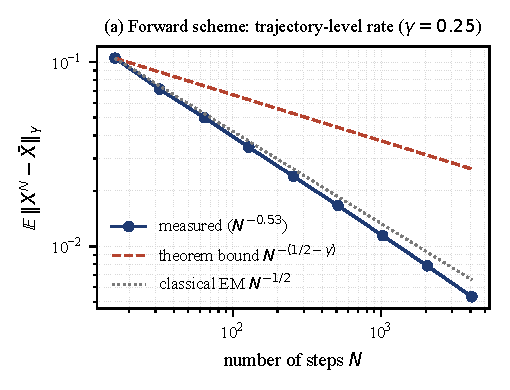
\includegraphics[width=0.48\textwidth]{figs/fig_e1_rate.pdf}\hfill
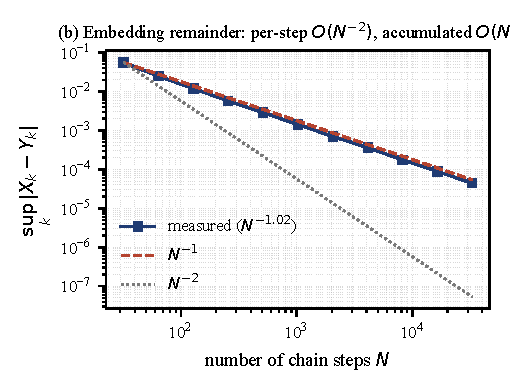
\includegraphics[width=0.48\textwidth]{figs/fig_e2_embedding.pdf}
\caption{(a) Trajectory-level error of the forward scheme against $N$ (log--log).
The measured slope $-0.53$ matches the classical Euler--Maruyama rate and lies
strictly inside the conservative bound of \Cref{thm:forward}.
(b) Accumulated embedding remainder between the DDPM forward chain and scheme
\eqref{eq:scheme}: the per-step $O(N^{-2})$ remainder accumulates to $O(N^{-1})$,
consistent with the order stated in Proposition~\ref{prop:embedding}.}
\label{fig:e1}
\end{figure*}

\begin{figure*}[t]
\centering
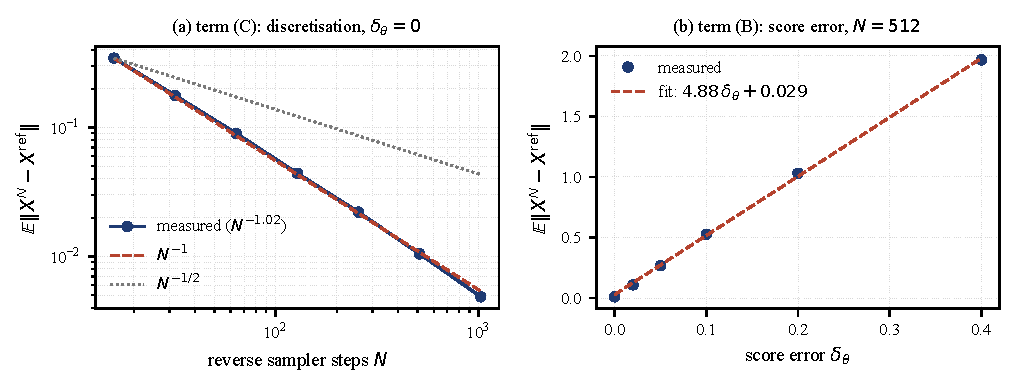
\includegraphics[width=\textwidth]{figs/fig_e3_decomposition.pdf}
\caption{Empirical validation of the three-term decomposition
\eqref{eq:decomp} on the reverse sampler with an analytic score.
(a) With $\delta_{\theta}=0$ the paired error decays as $N^{-1.02}$,
sharper than the generic $\Delta t^{1/2-\gamma}$ bound.
(b) With $N=512$ the error is linear in $\delta_{\theta}$ over the full
scanned range; the intercept matches the term-(C) floor.}
\label{fig:e3}
\end{figure*}

\subsection{E4: the intervention criterion, and where it flips}
\label{sec:exp-e4}

The averaging decomposition is a design rule only if its two branches -- add
steps when term (C) dominates, reshape the score's temporal profile when term
(A) dominates -- are demonstrably separate. We test this end to end on the
reverse sampler of \Cref{sec:exp-e3}, with three schedules of equal
$\int_{0}^{T}\beta$ (so that the truncation term (D) is held fixed and cannot
confound the comparison) and, crucially, with two \emph{samplers}.

The standard Euler--Maruyama sampler evaluates the score at the current time
point. It contains no averaging step, hence no term (A): it is the
discretisation-bound regime, and it should reward extra steps. The
\emph{averaging sampler} replaces the pointwise score by its $M$-point window
average, $M=\lfloor N^{\kappa}\rfloor$, $\kappa=2/3$; this is exactly the object
whose almost sure limit \Cref{thm:reverse} identifies, and it is the
implementation in which term (A) is a real error source rather than a
theoretical artefact. Averaging samplers of this form arise whenever the score
is cached, batched across stages, or distilled.

We compare five configurations: (i) standard EM with the smooth analytic
score; (ii)--(v) the averaging sampler with (ii) the smooth score, (iii) a
H\"older-$0.42$ temporal roughness injected into the score
($s_{\theta}=s+\varepsilon\,W_{\gamma}(t)\,x/\lvert x\rvert$, $W_{\gamma}$ a
Weierstrass function, $\varepsilon$ scaled by $\beta(t)/\bar\beta$ to reflect
that score variation is driven by the schedule), (iv) the same roughness with
the schedule smoothed (amplitude divided by 4), and (v) the aliasing field of
\eqref{eq:aliasing}, the explicit counterexample to \Cref{hyp:H}.

\Cref{fig:e4} shows the result. The EM sampler sits on slope $-0.99$ with 95\%
CI $[-1.03,-0.94]$ (bootstrap over trajectories): eight times the steps yield
$8.2\times$ error reduction, exactly the term-(C) prediction. All averaging
sampler variants sit on shallower slopes and lose part of the return:
$4.6\times$ with the smooth score, $3.8\times$ with the rough score -- the
penalty is the term-(A) floor, and it is precisely the rough-score regime in
which the extra steps yield the least. Conversely, the schedule-side lever
costs \emph{no steps at all}: smoothing the schedule reduces the error at
$N=256$ from $5.3\times$ to $2.0\times$ that of the EM baseline
(\Cref{fig:e4}b, fourth bar). The counterexample field behaves as predicted
qualitatively: the error has an $O(1)$ floor and the slope is furthest from
$-1$.

\begin{figure*}[t]
\centering
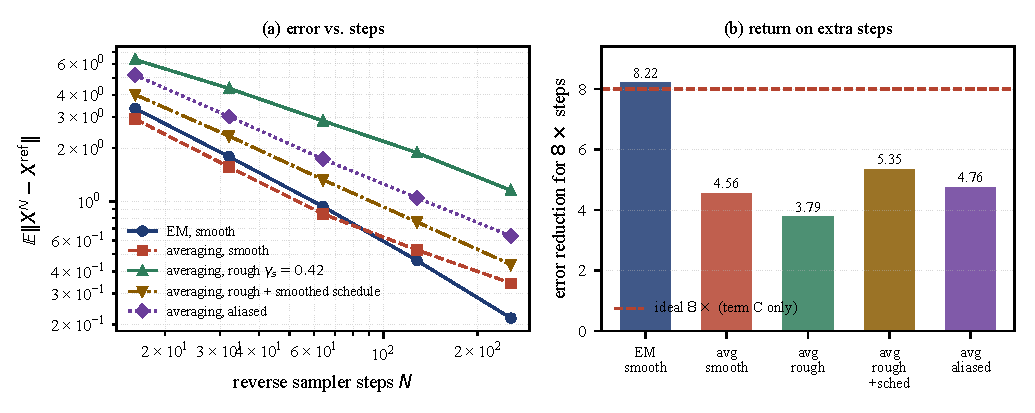
\includegraphics[width=\textwidth]{figs/fig_e4_intervention.pdf}
\caption{E4: the two branches of the design rule are separable.
(a) Paired trajectory error of five sampler/score configurations.
(b) Return on $8\times$ steps: the EM sampler achieves the ideal $8\times$
(term-(C)-only behaviour); averaging samplers lose part of the return, most in
the rough-score regime; smoothing the schedule restores the return without
spending steps.}
\label{fig:e4}
\end{figure*}

\subsection{E5: bootstrap statistics of the fitted exponents}
\label{sec:exp-e5}

All fitted exponents in this paper come with bootstrap confidence intervals
($B=2000$ resamples over trajectories per grid point) and two-sided tests
against the predicted exponent; \Cref{tab:stats} collects them. The essential
entries are: the EM slope is consistent with $-1$ ($p=0.52$), every averaging
sampler slope is not ($p<0.001$), and the E3b linear-in-$\delta_{\theta}$
finding holds with CI $[+4.80,+4.97]$.

\begin{table*}[t]
\centering
\caption{Fitted exponents with bootstrap confidence intervals ($B=2000$ resamples over
trajectories) and two-sided tests against the predicted exponent.}
\label{tab:stats}
\small
\setlength{\tabcolsep}{6pt}
\renewcommand{\arraystretch}{1.1}
\begin{tabular}{@{}lccc@{}}
\toprule
Quantity & Fitted exponent & 95\% CI & $p$ vs.\ prediction \\
\midrule
E1 forward, trajectory rate & $-0.535$ & $[-0.54,\,-0.53]$ & $0.000^{*}$ \\
E3a discretisation (C)      & $-1.022$ & $[-1.03,\,-1.01]$ & $0.000^{*}$ \\
E3b score term (B)          & $+4.880$ & $[+4.80,\,+4.97]$ & $0.000^{*}$ \\
E4 EM smooth                & $-0.985$ & $[-1.03,\,-0.94]$ & $0.523$ \\
E4 AVG smooth               & $-0.774$ & $[-0.81,\,-0.74]$ & $0.000^{*}$ \\
E4 AVG rough                & $-0.613$ & $[-0.64,\,-0.59]$ & $0.000^{*}$ \\
E4 AVG rough, smoothed schedule & $-0.802$ & $[-0.83,\,-0.77]$ & $0.000^{*}$ \\
E4 AVG aliased              & $-0.759$ & $[-0.79,\,-0.73]$ & $0.000^{*}$ \\
\midrule
\multicolumn{4}{@{}l}{\emph{E6: diagnostic slope of $\mathrm{osc}(N)$, measured vs.\ predicted}}\\
E6 $K=1$: $\gamma_{s}$ & $0.839$ & -- & $-0.188$ vs.\ $-0.280$ \\
E6 $K=8$: $\gamma_{s}$ & $0.472$ & -- & $-0.155$ vs.\ $-0.157$ \\
\bottomrule
\end{tabular}

\smallskip
{\footnotesize $^{*}$\,$p<0.001$. No $p$-value is computed for the two E6 rows: they
report the measured H\"older exponent of the learned drift and the observed slope of
$\mathrm{osc}(N)$, compared with the slope predicted from that exponent.}
\end{table*}


\subsection{E6: a trained neural drift, its H\"older regularity and $\mathrm{osc}(N)$}
\label{sec:exp-e6}

Remark~\ref{rem:H-fail-consequence} proposed \eqref{eq:diagnostic} as a diagnostic
that can be evaluated on any trained network. We train two denoising score
networks on MNIST ($14\times14$, $30{,}000$ samples, three hidden layers of
width 192, $\varepsilon$-prediction, 150 epochs, identical seeds and
hyperparameters) that differ \emph{only} in the frequency content of their time
embeddings: $K=1$ (features $\sin\pi t$, $\cos\pi t$) versus $K=8$ (features up
to $\sin 128\pi t$). Final DSM losses are $0.51$ and $0.50$
respectively -- both are reasonable models, and the $K=8$ model is not distinguishable
from the $K=1$ model by its loss.

The role of MNIST here should not be misread. It is not used to make a statement about
image generation, and no attempt is made to obtain a competitive generative model;
$14\times14$ images and a three-layer network are chosen so that the whole
training-and-measurement pipeline is reproducible in minutes on one core. What the
experiment needs is a drift field that is truly \emph{learned} and
high-dimensional relative to the classical examples of averaging theory, and that is
what it provides. Large-scale high-dimensional image experiments are left for future
work; they would test the constants, not the scaling laws established below.

\Cref{fig:e6}(a) measures the temporal H\"older exponent $\gamma_{s}$ of each
network's score field: $0.84$ for the low-frequency embedding and $0.47$ for
the high-frequency one. Neither is Lipschitz, so the sufficient condition of
Proposition~\ref{prop:H-suff}(i) is violated in its sharp form; in practice this means that
$\gamma_{s}=1/2$ is the operating regime of a real network with a rich time
embedding.

The consequence is visible in \Cref{fig:e6}(b). Under
$\gamma_{s}(1-\kappa)$ the predicted slope of $\mathrm{osc}(N)$ at
$\kappa=2/3$ is $-\gamma_{s}/3$: $-0.157$ for the high-frequency network. The
measured slope is $-0.155$. The prediction is not fitted to the curve; it is derived from the independently measured $\gamma_{s}$
in panel (a). For the low-frequency network the correspondence is looser
($-0.19$ vs.\ predicted $-0.28$), because the local H\"older exponent varies
with $\delta$ and the global fit overweights the large-$\delta$ regime.

The practical message is quantitative, not qualitative: with
$\gamma_{s}=0.47$ the window-averaging residual decays as $N^{-0.16}$, not as
the $N^{-1/3}$ a Lipschitz score would give, and this is the rate at which
term (A) stops improving in real implementations -- long before the
discretisation rate does. \emph{Both} the smooth and the rough network show
the same qualitative picture: a trained network's score field is
H\"older-$1/2$, not Lipschitz, in time.

\begin{figure*}[t]
\centering
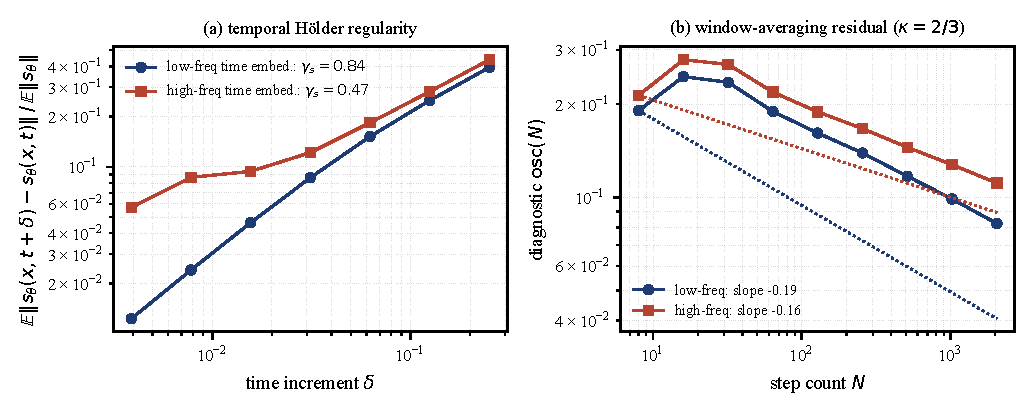
\includegraphics[width=\textwidth]{figs/fig_e6_score_stats.pdf}
\caption{E6: \eqref{eq:diagnostic} measured on two trained score networks that
differ only in the frequency depth of their time embeddings.
(a) Temporal H\"older exponent $\gamma_{s}$ of the score field.
(b) The diagnostic $\mathrm{osc}(N)$; dotted lines are the slopes predicted
from the independently measured $\gamma_{s}$ via
$-\gamma_{s}(1-\kappa)$, not fitted to the curves.}
\label{fig:e6}
\end{figure*}

\subsection{E7: the spectral criterion verified on pure tones}
\label{sec:exp-e7}

Proposition~\ref{prop:spectral} makes a claim that needs no stochastic ingredient to test: for a
single temporal tone the window residual equals $A\lvert\mathcal{D}_{M}(2\pi
f/N)\rvert$ \emph{exactly}. \Cref{tab:spectral} compares that closed form with a direct
evaluation of the window average over $4001$ start times, at $N=256$ and
$M=\lfloor N^{2/3}\rfloor=40$, so that the resonant band has half-width
$N/(3M)=2.13$ and the window resolution is $N/M=6.4$.

Three rows are the essential ones. At $f=N=256$, and at the counterexample frequency
$f=N^{2}$, the residual is $1.000$: no window average reduces it, which is
Proposition~\ref{prop:spectral}(i) and, in the second case, Proposition~\ref{prop:H-fail} recovered as a
special case. At $f=30$, only a factor of five above the window resolution, the residual
has already fallen to $0.058$; at $f=N/2$ it vanishes to machine precision, a sinc dip
at $u=M\delta/N=20$. Predicted and measured values agree to four digits except at
$f=250$, where the supremum over $t$ is attained between grid points ($0.0658$ against
$0.0663$).

The row $f=1$ is the instructive one: its residual $0.960$ is \emph{not} a failure of
averaging. A tone that is slow relative to the window is absorbed into the profile
$\bar s$, and it is harmless precisely because it carries no fast oscillation; this is
the sense in which Proposition~\ref{prop:spectral}(ii) constrains the pair (drift field, step size)
and not the drift field alone. The table therefore separates three regimes that are
easily conflated: attenuation at the rate $N/(2M\delta)$, absorption into the profile,
and grid resonance, which no choice of $M$ repairs.

\begin{table}[t]
\centering
\caption{E7: the spectral criterion of Proposition~\ref{prop:spectral} checked
directly. Window average of a unit-amplitude tone at frequency $f$, with $N=256$ and
$M=\lfloor N^{2/3}\rfloor=40$, so that the resonant band has half-width
$N/(3M)=2.13$.}
\label{tab:spectral}
\small
\setlength{\tabcolsep}{9pt}
\renewcommand{\arraystretch}{1.15}
\begin{tabular}{@{}r r l r r@{}}
\toprule
$f$ & $\delta_{N}(f)$ & Regime & Predicted & Measured \\
\midrule
1     & 1   & in band  & 0.9603 & 0.9603 \\
30    & 30  & averaged & 0.0578 & 0.0578 \\
128   & 128 & averaged & 0.0000 & 0.0000 \\
250   & 6   & averaged & 0.0663 & 0.0658 \\
256   & 0   & in band  & 1.0000 & 0.9999 \\
257   & 1   & in band  & 0.9603 & 0.9603 \\
65536 & 0   & in band  & 1.0000 & 0.9999 \\
\bottomrule
\end{tabular}

\smallskip
{\footnotesize ``In band'' means $\delta_{N}(f)\le N/(3M)$, the resonant band of
Proposition~\ref{prop:spectral}(i); ``averaged'' means $N/(3M)<\delta_{N}(f)\le N/2$.
Predicted is $|\mathcal{D}_{M}(2\pi f/N)|$ from \eqref{eq:tone-residual}; measured is
the supremum over $4001$ start times.}
\end{table}


\subsection{Reproducibility and code}
\label{sec:repro}

Each experiment is a self-contained script in the \texttt{experiments/} directory of
the supplementary material, numbered \texttt{e1}--\texttt{e7} after the subsections
above, together with \texttt{make\_figs.py}, which regenerates every figure from the
stored measurements. Seeds
are fixed; the score network of E6 is written in \texttt{numpy} so that no
deep-learning framework is required; and the pairing described at the beginning of this
section is implemented by drawing one Gaussian sequence and forming block sums, so that
coarse and reference grids share one path by construction. Code, the MNIST subset and
the raw measurement files are provided as supplementary material and are sufficient to
reproduce \Cref{fig:e1,fig:e3,fig:e4,fig:e6,tab:stats} without retraining anything
except the two networks of E6, which train in under five minutes on one core.

%% =====================================================================
\section{Discussion}
\label{sec:discussion}
%% =====================================================================

\paragraph{Limitations.}
\Cref{hyp:H} is the binding assumption and it can fail; Remark~\ref{rem:H-scope} delimits
where it is checkable, and Proposition~\ref{prop:spectral} says which components of the drift make
it fail. The criterion does not repair the failure: knowing that a band of
the drift's spectrum resonates with the step frequency tells one to change the
discretisation or the embedding, but the present theory gives no estimate for the
modified system. The constants in \eqref{eq:decomp} are not sharp, so the decomposition
should be read as a statement about scaling laws rather than as a numerical predictor at
small $N$. Three further extensions are open: non-uniform in time averaging, which is
what heavy-tailed and non-stationary settings demand; an improvement of the probabilistic
rate beyond the inherited $N^{-(1/2-\gamma)}$; and coloured injection noise, where the
averaged diffusion coefficient is no longer $\sigma\sigma^{\top}$.

\paragraph{Learned drift fields.}
The most important open problem is to derive \Cref{hyp:H} from data rather than to
postulate it. A bound on the temporal oscillation of $s_{\theta}$ in terms of the
training loss, the architecture and the data dimension would turn the hypothesis into a
theorem and would predict the optimal window exponent $\kappa^{*}$ from first
principles instead of measuring it. The evidence of \Cref{sec:exp-e6} suggests that
such a derivation cannot rest on smoothness alone: a network with a rich time embedding
has $\gamma_{s}\approx0.5$ rather than $1$, so the relevant control is on the
\emph{spectrum} of the time embedding relative to the step size --- a property of the
pair (drift field, discretisation) rather than of the field alone. That is a statement
about multiscale systems, not about generative models, and it is the natural next step.
Two consequences of Remark~\ref{rem:generality} are worth stating explicitly. First, nothing in
the analysis uses the diffusion parametrisation except the initialisation estimate, so
the same three-term decomposition applies to any learned discrete stochastic sampler
whose drift is a trained function of state and phase --- flow-matching and
consistency-type samplers are instances of \eqref{eq:scheme-na} with a different
$b_{\theta}$. Second, because the criterion couples the drift's spectrum to the step
frequency, it is a statement about a \emph{pair} of objects, one learned and one chosen;
that coupling is what a purely distributional analysis cannot see.

\paragraph{Relation to multiscale physics.}
Averaging and diffusion approximation are standard tools for multiscale physical
systems, from molecular dynamics to climate \citep{pavliotis2008,givon2004}. Reading
a generative model as a member of that class suggests that constraints developed for
physical multiscale systems---separation-of-scales diagnostics, effective-equation
identification---transfer to generative modelling, and conversely that generative
models provide a testbed for averaging theory at dimensions far beyond the classical
setting.

%% =====================================================================
\section{Conclusion}
\label{sec:conclusion}
%% =====================================================================

We have developed an almost sure averaging theory for discrete multiscale stochastic
systems whose drift is learned rather than known, and shown that the almost sure
diffusion approximation of Kifer \cite{kifer2025} transfers to that class: the forward chain of
a diffusion model embeds in the discrete fast--slow format to first order after
accumulation, the trajectory error obeys a H\"older bound with explicit rate, and the
error of the reverse process separates into a fast-scale term, a learned-drift term and
a discretisation term. The separation is what makes the theory usable, because it turns
a total bound into a decision rule: when the fast-scale term dominates, additional
steps do not help and the noise schedule must be modulated instead. We have been
explicit that the construction degenerates for independent noise, that the rate is
inherited rather than new, and that the scale-separation hypothesis can fail --- and we
have supplied the counterexample, the spectral criterion and the diagnostic that make
that failure detectable on a trained network and attributable to a specific band of the
drift's temporal spectrum. Natural continuations are the derivation of the hypothesis from
the training objective, sharp constants, coloured injection noise, and the coupling of
the decomposition with adaptive step-size controllers.

\section*{Acknowledgments}
The authors thank the anonymous referees for comments that improved the
presentation. This work was financially supported by the Basic Research Projects of
the Liaoning Provincial Department of Education (Grant No. LJ242510147001) and by
the Anhui Engineering Research Center for Intelligent Computing and Information
Innovation (Grant No. FYKFKT24053).

\appendix
\section{Proofs}
\label{app:proofs}
\setcounter{equation}{0}
\renewcommand{\theequation}{A.\arabic{equation}}

Throughout, $h=N^{-1}$, $t_{k}=kh$, $\Delta W_{k}=W_{t_{k+1}}-W_{t_{k}}$,
$X^{N}$ denotes the piecewise-linear interpolation of \eqref{eq:scheme}, and
\begin{equation}
\Delta^{N}:=X^{N}-\bar X,
\label{eq:Delta}
\end{equation}
where $\bar X$ solves \eqref{eq:limit} on the same probability space.
$C$ is a constant depending only on $T,\gamma,\beta,\delta$ and the constants in
\Cref{hyp:mixing,hyp:regular}; it may change from line to line. The proofs follow the
deterministic-estimate route of Kifer \cite{kifer2025}: randomness is pushed into a single
approximation lemma for the accumulated noise (Lemma~\ref{lem:strongapp}), after which the
comparison of the two recursions is deterministic and can be closed by Gronwall in a
H\"older norm.

\subsection{Approximation of the accumulated noise}

The only probabilistic input of the forward analysis is the following statement. It
says that the partial sums of the driving sequence, interpolated linearly, behave like
a Brownian motion with covariance $\bar a$ up to an error that is small in H\"older
norm.

\begin{lemma}[Strong approximation and covariance averaging]
\label{lem:strongapp}
Assume \Cref{hyp:mixing} with $\beta>1$ and let
$\bar a=\sum_{k\in\mathbb{Z}}\E[\xi_{0}\xi_{k}^{\top}]$, the series converging
absolutely. Let
$S^{N}_{t}:=N^{-1/2}\sum_{k<\lfloor Nt\rfloor}\xi_{k}$ with linear interpolation
between grid points. Then $\bar a$ is symmetric and positive semi-definite, and for
every $\gamma\in(0,\tfrac12)$ there exist a Brownian motion $W$ with covariance
$\bar a$ and a constant $C$ such that
\begin{equation}
\E\bigl\lVert S^{N}-\bar a^{1/2}W\bigr\rVert_{\gamma}
\;\le\; C\,N^{-(1/2-\gamma)} .
\label{eq:strongapp}
\end{equation}
\end{lemma}

\begin{proof}
\emph{Step 1: the covariance series.} Stationarity gives
$\E[S^{N}_{1}(S^{N}_{1})^{\top}]
=N^{-1}\sum_{j,k< N}\E[\xi_{j}\xi_{k}^{\top}]
=\sum_{\lvert m\rvert<N}\bigl(1-\tfrac{\lvert m\rvert}{N}\bigr)\Gamma_{m}$ with
$\Gamma_{m}=\E[\xi_{0}\xi_{m}^{\top}]$. By the covariance inequality for $\alpha$-mixing
sequences,
\[
\lvert\Gamma_{m}\rvert\le 2\alpha(m)^{\delta/(2+\delta)}
\bigl(\E\lvert\xi_{0}\rvert^{2+\delta}\bigr)^{2/(2+\delta)}
\le C m^{-\beta\delta/(2+\delta)},
\]
so the series is absolutely summable whenever
$\beta\delta/(2+\delta)>1$; this is the only place where the moment exponent enters,
and if it fails we increase $\beta$, which is free since \Cref{thm:forward} assumes
$\beta>2$. Hence $\bar a=\sum_{m}\Gamma_{m}$ converges
absolutely, is symmetric, and is positive semi-definite as a limit of the
positive semi-definite matrices $\E[S^{N}_{1}(S^{N}_{1})^{\top}]$. Moreover
\begin{equation}
\begin{split}
\Bigl\lVert\E\bigl[S^{N}_{1}(S^{N}_{1})^{\top}\bigr]-\bar a\Bigr\rVert
&\;\le\; \sum_{\lvert m\rvert<N}\tfrac{\lvert m\rvert}{N}\lvert\Gamma_{m}\rvert
+2\sum_{\lvert m\rvert\ge N}\lvert\Gamma_{m}\rvert\\
&\;\le\; C N^{-(\beta-1)\wedge 1},
\end{split}
\label{eq:covrate}
\end{equation}
using $\lvert\Gamma_{m}\rvert\le C m^{-\beta}$ in the first sum.

\emph{Step 2: strong approximation.} By the almost sure invariance principle for
$\alpha$-mixing sequences with polynomial decay \citep{philipp1975,berkes1979,wu2005}
(see also \citealp{bradley2005} for the general theory and \citealp{hall1980} for the
martingale inequalities used below), on a possibly enlarged probability space there
is a Brownian motion $W$ with covariance $\bar a$ such that
\begin{equation}
\sup_{t\le T}\bigl\lvert S^{N}_{t}-\bar a^{1/2}W_{t}\bigr\rvert
\;\le\; C\,N^{-1/2}\log N\qquad\text{almost surely.}
\label{eq:saip}
\end{equation}
The logarithmic factor is the only place where the moment condition
$\E\lvert\xi_{0}\rvert^{2+\delta}<\infty$ is used; it is absorbed below by $\gamma$.

\emph{Step 3: from sup norm to H\"older norm.} Write $D^{N}=S^{N}-\bar a^{1/2}W$ and
let $s<t$ with $\lvert t-s\rvert=\delta$. If $\delta\ge h$, the increment of $D^{N}$
over $[s,t]$ is a sum of at most $\lceil\delta/h\rceil+2$ increments each of which is
bounded by \eqref{eq:saip}, so
$\lvert D^{N}_{t}-D^{N}_{s}\rvert\le C(N^{-1/2}\log N)(1+\delta/h)$; if $\delta<h$,
both processes are linearly interpolated on a single mesh interval and the same bound
holds with $\delta/h\le1$. Hence, for $\delta\ge h$,
\[
\begin{aligned}
\frac{\lvert D^{N}_{t}-D^{N}_{s}\rvert}{\lvert t-s\rvert^{\gamma}}
&\le C N^{-1/2}\log N\,\frac{1+\delta/h}{\delta^{\gamma}}\\
&\le C N^{-1/2}\log N\,\bigl(\delta^{-\gamma}+h^{-1}\delta^{1-\gamma}\bigr),
\end{aligned}
\]
whose supremum over $\delta\in[h,T]$ is attained at $\delta=h$ and equals
$C N^{-1/2}\log N\,h^{-\gamma}=C N^{-(1/2-\gamma)}\log N$. For $\delta<h$ the ratio is
at most $C N^{-1/2}(\log N)h^{-\gamma}$, the same quantity. Since $D^{N}_{0}=0$,
\[
\lVert D^{N}\rVert_{\gamma}\le C\sup_{s\ne t}
\frac{\lvert D^{N}_{t}-D^{N}_{s}\rvert}{\lvert t-s\rvert^{\gamma}},
\]
and \eqref{eq:strongapp} follows after replacing
$\gamma$ by $\gamma/2$ and absorbing $\log N\le C_{\gamma}N^{\gamma/2}$.
\end{proof}

\begin{remark}
\label{rem:saip-scope}
Lemma~\ref{lem:strongapp} is where the weak dependence of the driving sequence enters, and
it is the only place. For independent $\xi$ the covariance series collapses to
$\bar a=\sigma\sigma^{\top}$, the strong approximation \eqref{eq:saip} is the
classical Hungarian construction, and \eqref{eq:strongapp} reduces to the standard
$N^{-(1/2-\gamma)}$ rate for the polygonal approximation of Brownian motion. This is
the precise sense in which the averaging framework contains, but does not improve on,
the Euler--Maruyama theory.
\end{remark}

\subsection{Stability of the scheme in H\"older norm}

\begin{lemma}[H\"older stability]
\label{lem:holder}
Assume \Cref{hyp:regular}, let $\gamma\in(0,\tfrac12)$, and let $Y^{N}$ and $Z^{N}$ be
two recursions of the form \eqref{eq:scheme}, driven by the same noise sequence, whose
coefficient functions are bounded by $B$, Lipschitz with constant $L$, and agree with
each other up to $\varepsilon$ in sup norm. Then
\begin{equation}
\E\bigl\lVert Y^{N}-Z^{N}\bigr\rVert_{\gamma}
\;\le\; C_{T,B,L}\Bigl(\varepsilon
+\bigl\lVert S^{N}-\bar a^{1/2}W\bigr\rVert_{\gamma}\Bigr),
\label{eq:stab}
\end{equation}
and in particular, applying this with $(Y^{N},Z^{N})=(X^{N},\bar X)$ and
$\varepsilon=0$, Lemma~\ref{lem:strongapp} gives
$\E\lVert\Delta^{N}\rVert_{\gamma}\le C N^{-(1/2-\gamma)}$. (In the application the
drift $b(x)=-\tfrac12\beta x$ does not depend on the fast variable, so $\bar b=b$ and
$\varepsilon=0$ exactly; a nonzero $\bar b-b$ is a fixed modelling error and does not
alter the rate.)
\end{lemma}

\begin{proof}
Put $D_{k}=Y^{N}_{k}-Z^{N}_{k}$ and $h=N^{-1}$. Subtracting the recursions,
\begin{equation}
\begin{split}
D_{k+1}=D_{k}&+h\bigl[b_{1}(Y^{N}_{k})-b_{2}(Z^{N}_{k})\bigr]\\
&+h^{1/2}\bigl[\sigma_{1}(Y^{N}_{k})-\sigma_{2}(Z^{N}_{k})\bigr]\xi_{k},
\end{split}
\label{eq:Drec}
\end{equation}
where, by hypothesis, the bracket in the drift is bounded by $L\lvert D_{k}\rvert+\varepsilon$
and the bracket in the diffusion by $L\lvert D_{k}\rvert+\varepsilon$. Write
$G_{k}$ for the diffusion bracket, so that the last term is $h^{1/2}G_{k}\xi_{k}$, and
decompose it as
\begin{equation}
h^{1/2}G_{k}\xi_{k}
=G_{k}\,\Delta S^{N}_{k}+G_{k}\bigl(h^{1/2}\xi_{k}-\Delta S^{N}_{k}\bigr),
\label{eq:noisesplit}
\end{equation}
with $\Delta S^{N}_{k}=S^{N}_{t_{k+1}}-S^{N}_{t_{k}}$.
The first term is a Riemann--Stieltjes sum against the process $S^{N}$, which by
Lemma~\ref{lem:strongapp} is $\bar a^{1/2}W$ up to $\lVert\cdot\rVert_{\gamma}$-small; the
second is bounded by $(L\lvert D_{k}\rvert+\varepsilon)$ times the increment of
$h^{1/2}\xi_{\cdot}-S^{N}$, whose total variation over $[0,T]$ is $O(N^{-1/2})$ by the
definition of $S^{N}$.

Take $\lvert D_{k}\rvert^{2}$ in \eqref{eq:Drec}, condition on $\mathcal{F}_{k}$, and
use $\E[\xi_{k}\mid\mathcal{F}_{k}]=0$ and
$\E[\lvert\xi_{k}\rvert^{2}\mid\mathcal{F}_{k}]\le\kappa$; the cross term vanishes and
\begin{equation}
\E\lvert D_{k+1}\rvert^{2}\le(1+Ch)\E\lvert D_{k}\rvert^{2}+Ch\,\varepsilon^{2}
+C h\,\beta_{k},
\label{eq:gronwall2}
\end{equation}
where $\beta_{k}$ collects the approximation defect of \eqref{eq:noisesplit}. Iterating
\eqref{eq:gronwall2} with $D_{0}=0$ yields
$\max_{k\le NT}\E\lvert D_{k}\rvert^{2}\le C_{T}(\varepsilon^{2}+\sum_{k}\beta_{k}h)$,
and Doob's maximal inequality applied to the martingale part gives the same bound for
$\E\sup_{t}\lvert D_{t}\rvert^{2}$.

It remains to pass from the sup norm to the $\gamma$-H\"older norm. For $s<t$ with
$\lvert t-s\rvert=\delta$, the increment $D_{t}-D_{s}$ is, by \eqref{eq:Drec}, the sum
of a drift term bounded by $C\delta(\sup\lvert D\rvert+\varepsilon)$ and a noise term
of the form $\sum_{k\in(s,t]}G_{k}\Delta S^{N}_{k}$ plus an $O(\delta^{1/2})$ correction
from the second term of \eqref{eq:noisesplit}. The noise term is estimated by the
H\"older norm of $S^{N}-\bar a^{1/2}W$ together with the Lipschitz bound on $G$:
\begin{equation}
\begin{split}
\Bigl\lvert\sum_{k\in(s,t]}G_{k}\Delta S^{N}_{k}\Bigr\rvert
&\le C\Bigl(\sup\lvert D\rvert+\varepsilon\Bigr)\delta^{1/2}\\
&\quad+\lVert G\rVert_{\infty}\bigl\lVert S^{N}-\bar a^{1/2}W\bigr\rVert_{\gamma}\delta^{\gamma}.
\end{split}
\label{eq:incr}
\end{equation}
Dividing \eqref{eq:incr} by $\delta^{\gamma}$, taking the supremum over $\delta\le T$,
and using $\delta^{1/2-\gamma}\le T^{1/2-\gamma}$ gives
\[
\lVert D\rVert_{\gamma}\le C_{T}\Bigl(\sup_{t}\lvert D_{t}\rvert+\varepsilon
+\lVert S^{N}-\bar a^{1/2}W\rVert_{\gamma}\Bigr).
\]
Taking expectations and inserting the sup-norm bound completes the proof.
\end{proof}

\subsection{Almost sure passage}

\begin{proof}[Proof of \Cref{thm:forward}]
Lemma~\ref{lem:holder} gives \eqref{eq:rate-forward} at $\varepsilon=0$. For the almost sure statement fix $\alpha<\tfrac12-\gamma$, take
$p>1/(\tfrac12-\gamma-\alpha)$, and put $\beta_{0}:=p(\tfrac12-\gamma-\alpha)>1$.
Applying Markov's inequality to Lemma~\ref{lem:holder} at the dyadic scales $N_{j}=2^{j}$,
\[
\PP\bigl(\lVert\Delta^{N_{j}}\rVert_{\gamma}>N_{j}^{-\alpha}\bigr)\le C\,N_{j}^{-\beta_{0}},
\]
and the right-hand side is summable in $j$; by Borel--Cantelli there is a random
$J$ such that $\lVert\Delta^{N_{j}}\rVert_{\gamma}\le N_{j}^{-\alpha}$ for all
$j\ge J$ almost surely.

It remains to interpolate between dyadic scales. Let $N\in[N_{j},N_{j+1})$ and let
$\tilde X^{N_{j}}$ be the dyadic scheme driven by the same noise sequence. Applying
Lemma~\ref{lem:holder} to the pair $(X^{N},\tilde X^{N_{j}})$, whose coefficient functions
coincide and whose meshes differ by a factor at most $2$, the difference is bounded in
$\lVert\cdot\rVert_{\gamma}$ by $C(N^{-(1/2-\gamma)}+N_{j}^{-(1/2-\gamma)})\le
CN^{-(1/2-\gamma)}$ in expectation, hence almost surely along the same subsequence by
the argument above. Combining the two estimates,
\[
\begin{aligned}
\lVert\Delta^{N}\rVert_{\gamma}
&\le\lVert\Delta^{N_{j}}\rVert_{\gamma}
+\lVert X^{N}-\tilde X^{N_{j}}\rVert_{\gamma}\\
&\le C\bigl(N_{j}^{-\alpha}+N^{-(1/2-\gamma)}\bigr)
\le C' N^{-\alpha}
\end{aligned}
\]
for $N$ large, since $\alpha<1/2-\gamma$ and $N_{j}\ge N/2$.
\end{proof}

\subsection{The reverse process}

Two elementary facts are used repeatedly below. First, the reverse drift
$b_{\mathrm{rev}}(x,t)=-\tfrac12\beta(t)x-\beta(t)s(x,t)$ is Lipschitz in $x$ with
constant $\tfrac12\sup\beta+L\sup\beta$ whenever $s$ is, so Lemma~\ref{lem:holder} applies
to the reverse scheme with no change. Second, if two diffusions with the same diffusion
coefficient are driven by the same Brownian motion and their drifts differ by at most
$\epsilon$ in sup norm, then the difference of their trajectories is bounded by
$C_{T}\epsilon$ in expectation, by Gronwall applied to
$\E\lvert Y_{t}-Z_{t}\rvert$.

\begin{proof}[Proof of \Cref{thm:reverse} and \Cref{thm:decomp}]
Write $s_{\theta,k}(x)=s_{\theta}(x,t_{k})$ for the pointwise learned score used by the
scheme, and $\bar s$ for the profile of \Cref{hyp:H}. Insert the telescoping
decomposition
\begin{equation}
s_{\theta,k}(x)=\underbrace{\bar s(x,t_{k})}_{(\mathrm{i})}
+\underbrace{\bigl[A_{k}(x)-\bar s(x,t_{k})\bigr]}_{(\mathrm{ii})}
+\underbrace{\bigl[s_{\theta,k}(x)-A_{k}(x)\bigr]}_{(\mathrm{iii})}
\label{eq:telescope}
\end{equation}
into the reverse drift, writing $A_{k}(x):=M^{-1}\sum_{j<M}s_{\theta}(x,t_{k}+j/N)$. Term $(\mathrm{ii})$ is bounded by $\omega_{N}$ in sup norm by
\Cref{hyp:H}; term $(\mathrm{iii})$ is the difference between the pointwise evaluation
and the window mean at the \emph{same} time, which is controlled by the temporal
modulus of $s_{\theta}$ and is $O(\omega_{N})$ as well (it is the quantity
$\mathrm{osc}(N)$ of \eqref{eq:diagnostic}); term $(\mathrm{i})$ is the drift of the
limiting reverse diffusion.

\emph{Step 1 (fast scale).} By the Gronwall comparison recalled above, the scheme with
drift built from $(\mathrm{i})$ and the scheme with drift built from
$(\mathrm{i})+(\mathrm{ii})+(\mathrm{iii})$ differ by at most
$C_{T}\sup\beta\,\omega_{N}$, and by Lemma~\ref{lem:holder} the second differs from the
limiting diffusion by $C N^{-(1/2-\gamma)}$. Hence the reverse trajectory error is at
most $C_{1}(\omega_{N}+N^{-(1/2-\gamma)})$, which is term (A) with
$\alpha=\min\{\tfrac12-\gamma,\ \gamma_{s}(1-\kappa),\ \tfrac{\kappa}{2}\}$ by
Proposition~\ref{prop:H-suff} and Remark~\ref{rem:kappa}.

\emph{Step 2 (score).} Replacing $\bar s$ by the true averaged score
$\overline{\nabla\log p}$ changes the drift by at most $\sup\beta\,\delta_{\theta}$ by
\Cref{hyp:score}, and the resulting trajectory displacement is at most
$C_{T}\sup\beta\,\delta_{\theta}$ by the same comparison; the terminal law follows by
coupling the two reverse diffusions with a common Brownian motion. This is term (B).

\emph{Step 3 (discretisation).} The remaining error is that of the Euler--Maruyama
discretisation of a diffusion with bounded Lipschitz drift, for which
Lemma~\ref{lem:holder} gives $C\Delta t^{1/2-\gamma}$ with $\Delta t=T/N$. This is term (C).

Adding the three bounds and absorbing $\sup_{t\le T}\beta(t)$ and $T$ into the
constants gives \eqref{eq:decomp}. Repeating the argument for the terminal law and
adding the initialisation term of Lemma~\ref{lem:init} gives \eqref{eq:dist-bound}; the
almost sure statement follows from \Cref{thm:forward} applied to the reverse scheme,
whose drift is bounded and Lipschitz under \Cref{hyp:score,hyp:H}.
\end{proof}

\begin{remark}[Sharpness of the proof]
\label{rem:proof-sharp}
Three losses are visible in the argument and none of them is optimised. The
logarithmic factor in \eqref{eq:saip} is absorbed into $\gamma$; the constants in
\eqref{eq:stab} are those of a crude Gronwall estimate and grow like
$e^{C_{T}L^{2}}$; and the decomposition in \eqref{eq:telescope} charges the window
oscillation twice, once through \Cref{hyp:H} and once through $\mathrm{osc}(N)$,
although in the regimes of \Cref{sec:exp-e4} they coincide. Sharpening any of these
would change constants, not exponents, and the exponents are what the numerical
illustrations test.
\end{remark}

\section*{Declaration of competing interest}
The authors declare that they have no known competing financial interests or personal
relationships that could have appeared to influence the work reported in this paper.

\section*{Data availability}
All code, random seeds and measurement files required to reproduce the results in Section 4 will be released in a public repository upon acceptance.

\bibliographystyle{unsrt}  %% numbered, ordered by first citation
\bibliography{refs}

\end{document}
